%!TEX root = main.tex
%!TeX TS-program = pdflatex
%!TeX encoding = UTF-8 Unicode
%!TeX spellcheck = fr
%!BIB TS-program = biber
% -*- coding: UTF-8; -*-
% vim: set fenc=utf-8
% Appendix A

\chapter{Figures} % Main appendix title

\label{Figures} % For referencing this appendix elsewhere, use \ref{AppendixA}

%%%%% Introduction %%%%%

%%%%% Matériel et méthodes %%%%%

\begin{table}
\resizebox{19cm}{!}{
\begin{tabular}{| p{4cm} || l | l | p{5cm} | l | l |}
\hline
Système d'explotation & Processeur & Mémoire vive & Carte graphique\\ \hline
Ubuntu 16.04.4 & Intel Xeon E5-1607 (3,1GHz) &  
40 GB & NVIDIA GeForce GTX1060\\ \hline
\end{tabular}
}
\caption[Tableau]{Matériel utilisé pour réaliser les modélisations
}
\label{tab:materiel}
\end{table}

\begin{figure}[th]
\centering
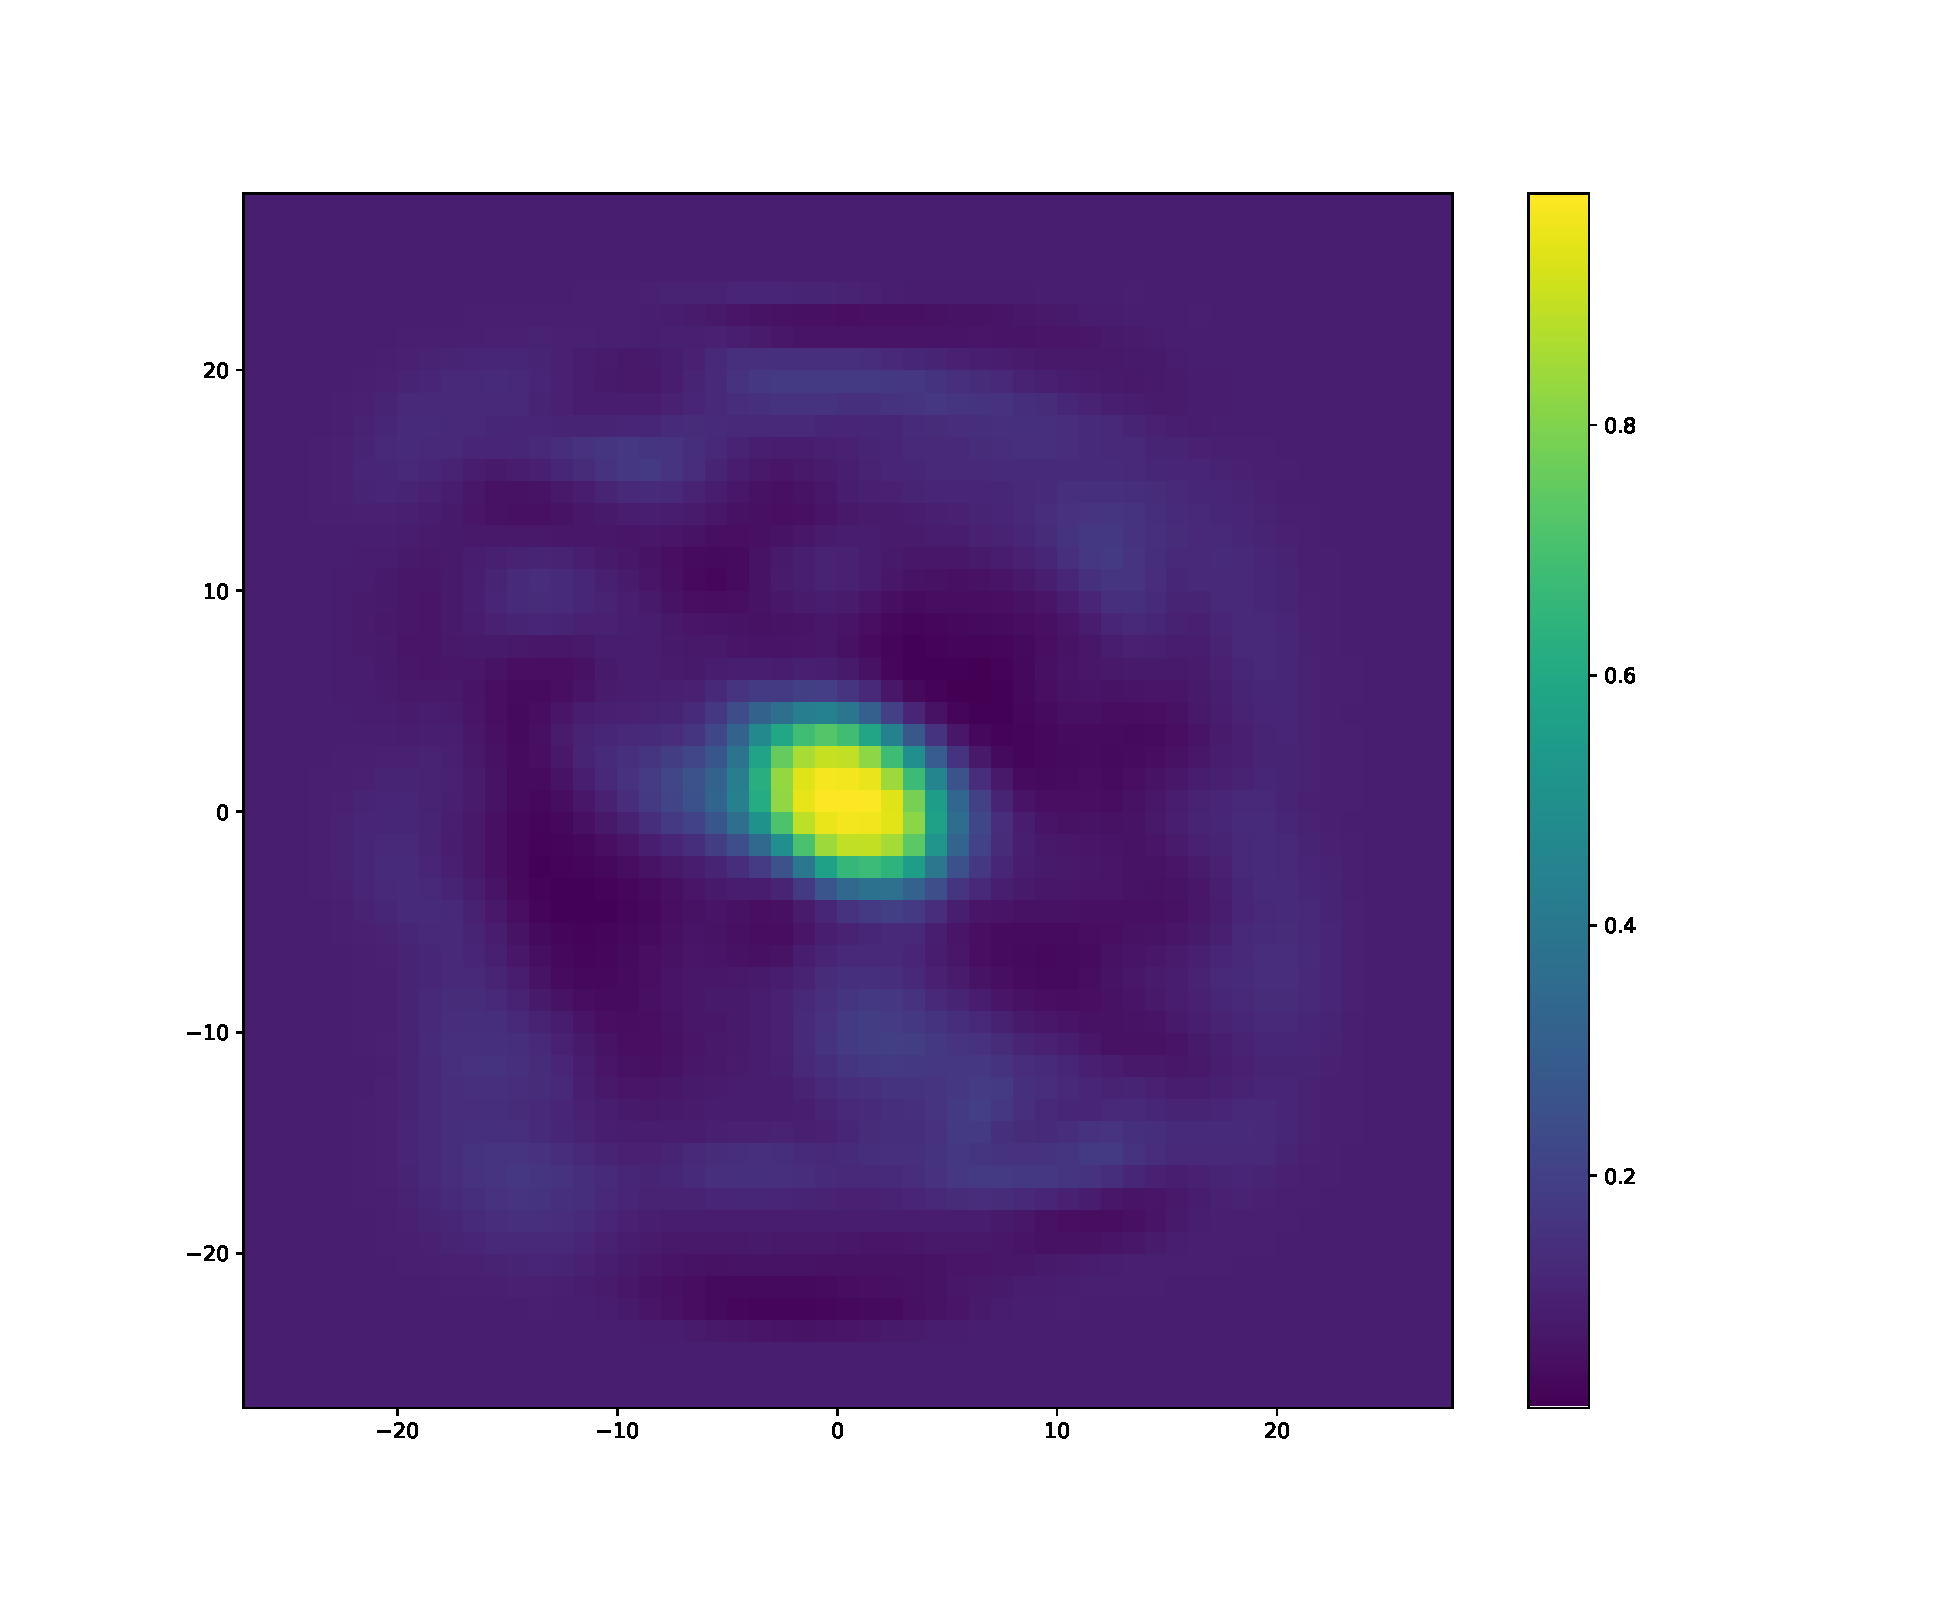
\includegraphics[scale=0.4]{Figures/accuracy}
\decoRule %puts an aesthetic horizontal line below the image
\caption[Figure]{Reconstruction en carte de chaleur ($55\times 55$ pixels) de la matrice de certitude}
\label{fig:accuracy}
\end{figure}

\begin{figure}[th]
\centering
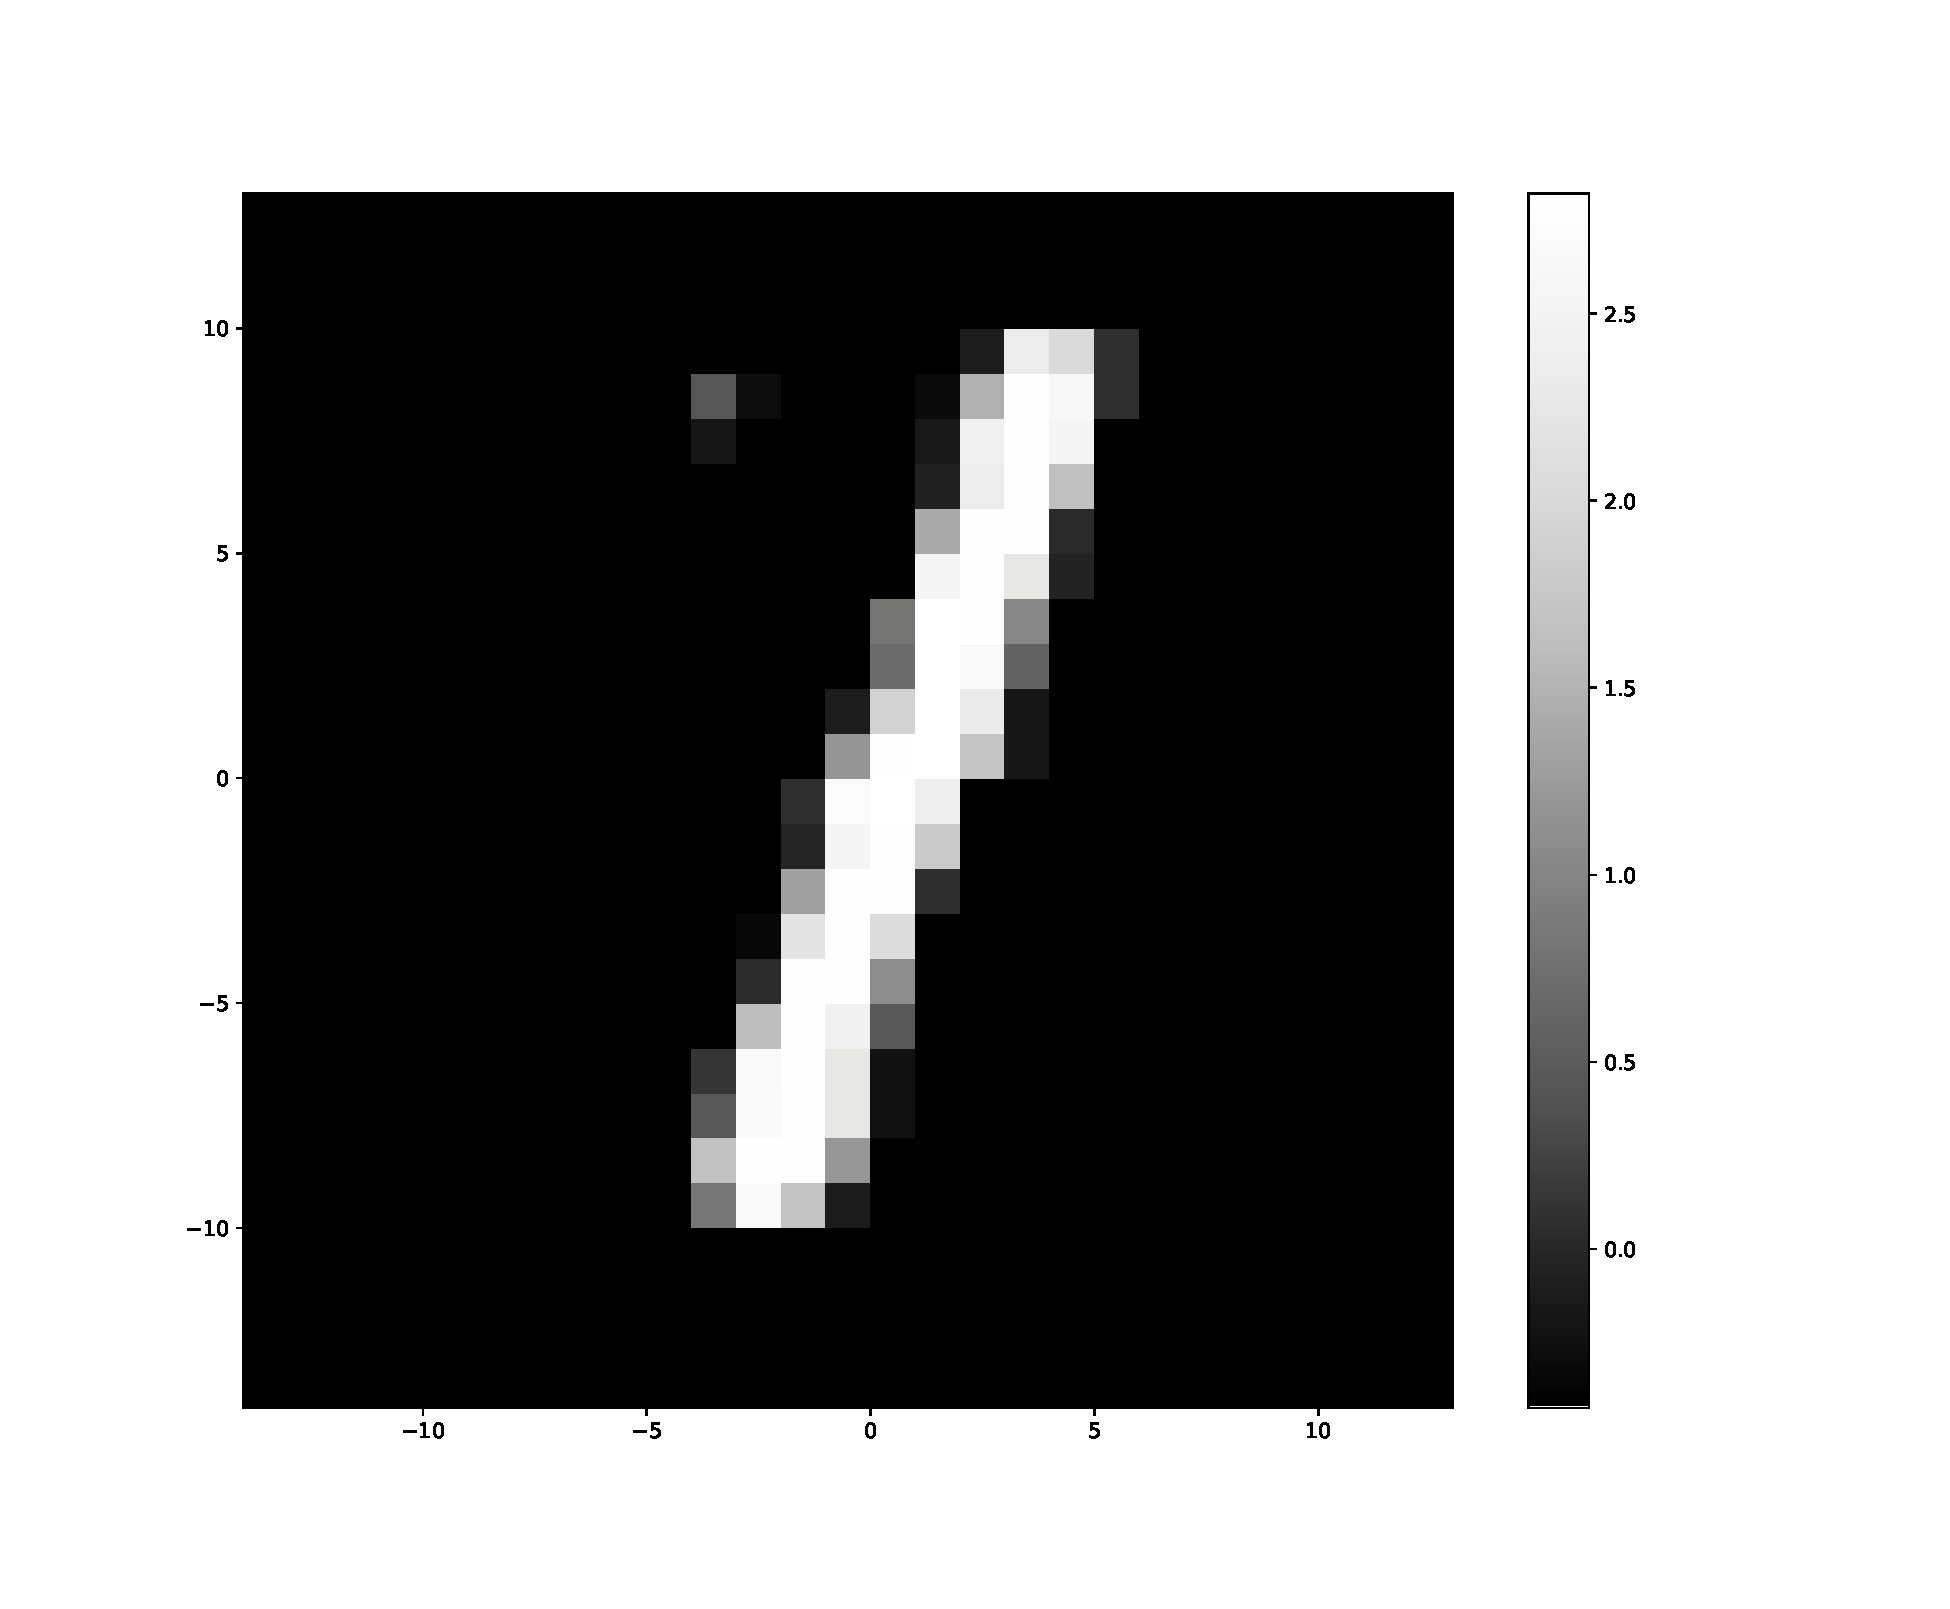
\includegraphics[scale=0.3]{Figures/MNIST_28}
\decoRule
\caption[Figure]{Reconstruction en carte de chaleur ($28\times 28$ pixels) d'une image provenant de la base de données MNIST}
\label{fig:MNIST_28}
\end{figure}

\begin{figure}[th]
\centering
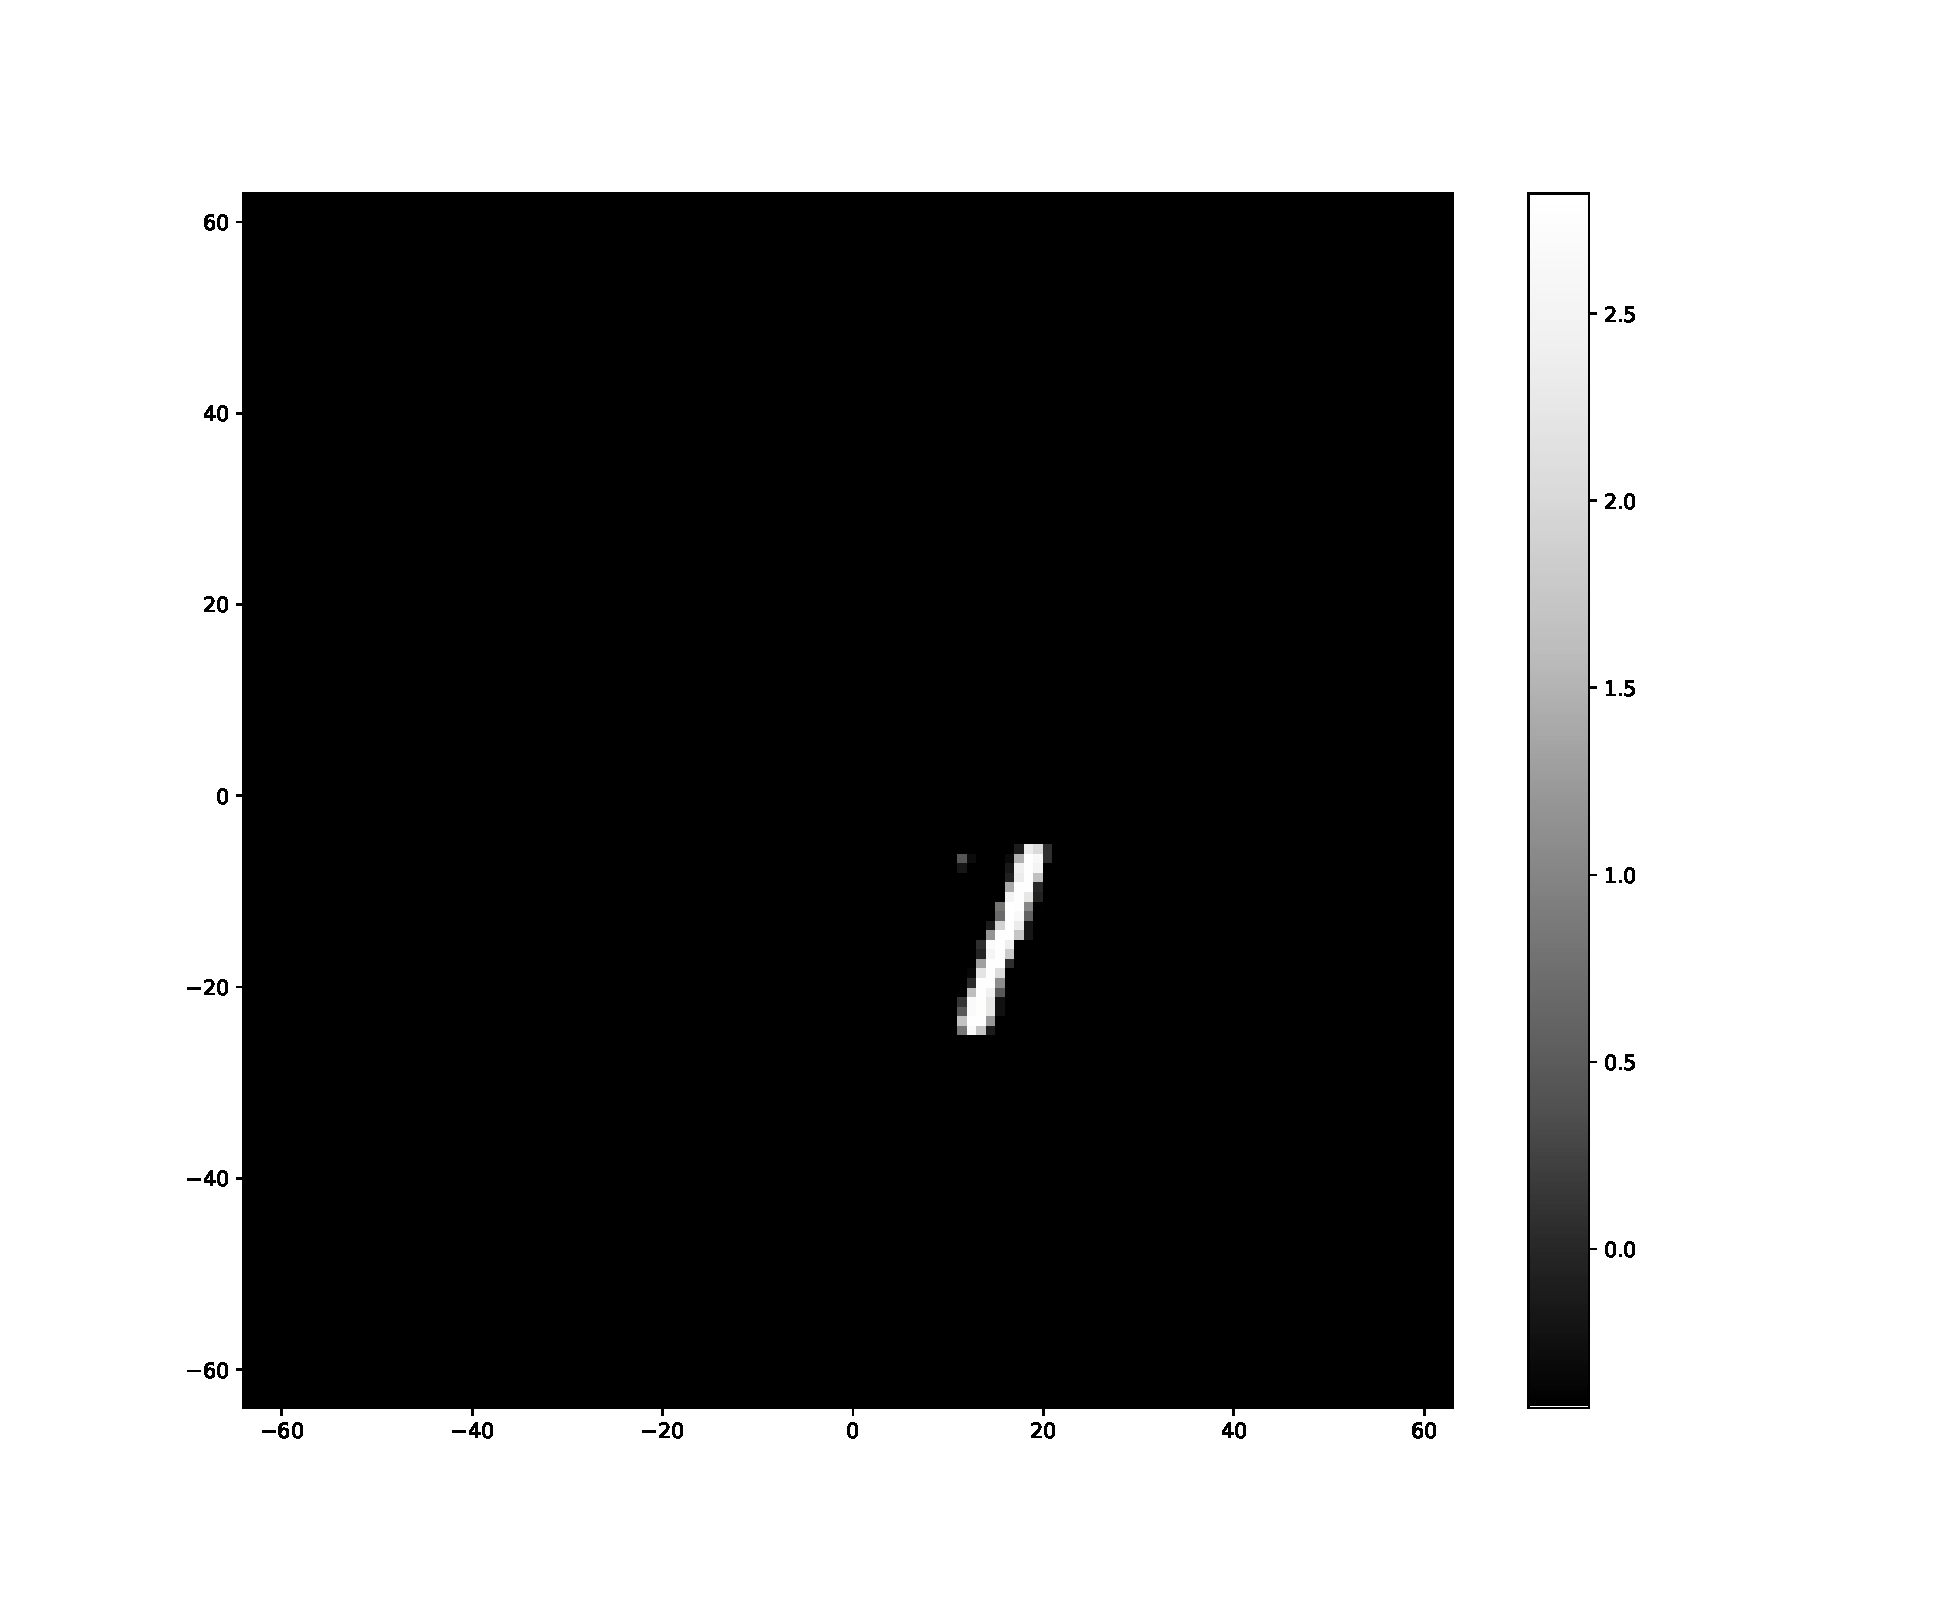
\includegraphics[scale=0.3]{Figures/mnist_128}
\decoRule
\caption[Figure]{Reconstruction en carte de chaleur d'une image provenant de la base de données MNIST, après transformation pour la placer dans une image de dimension $128\times 128$ pixels}
\label{fig:MNIST_128}
\end{figure}

\begin{figure}[th]
\centering
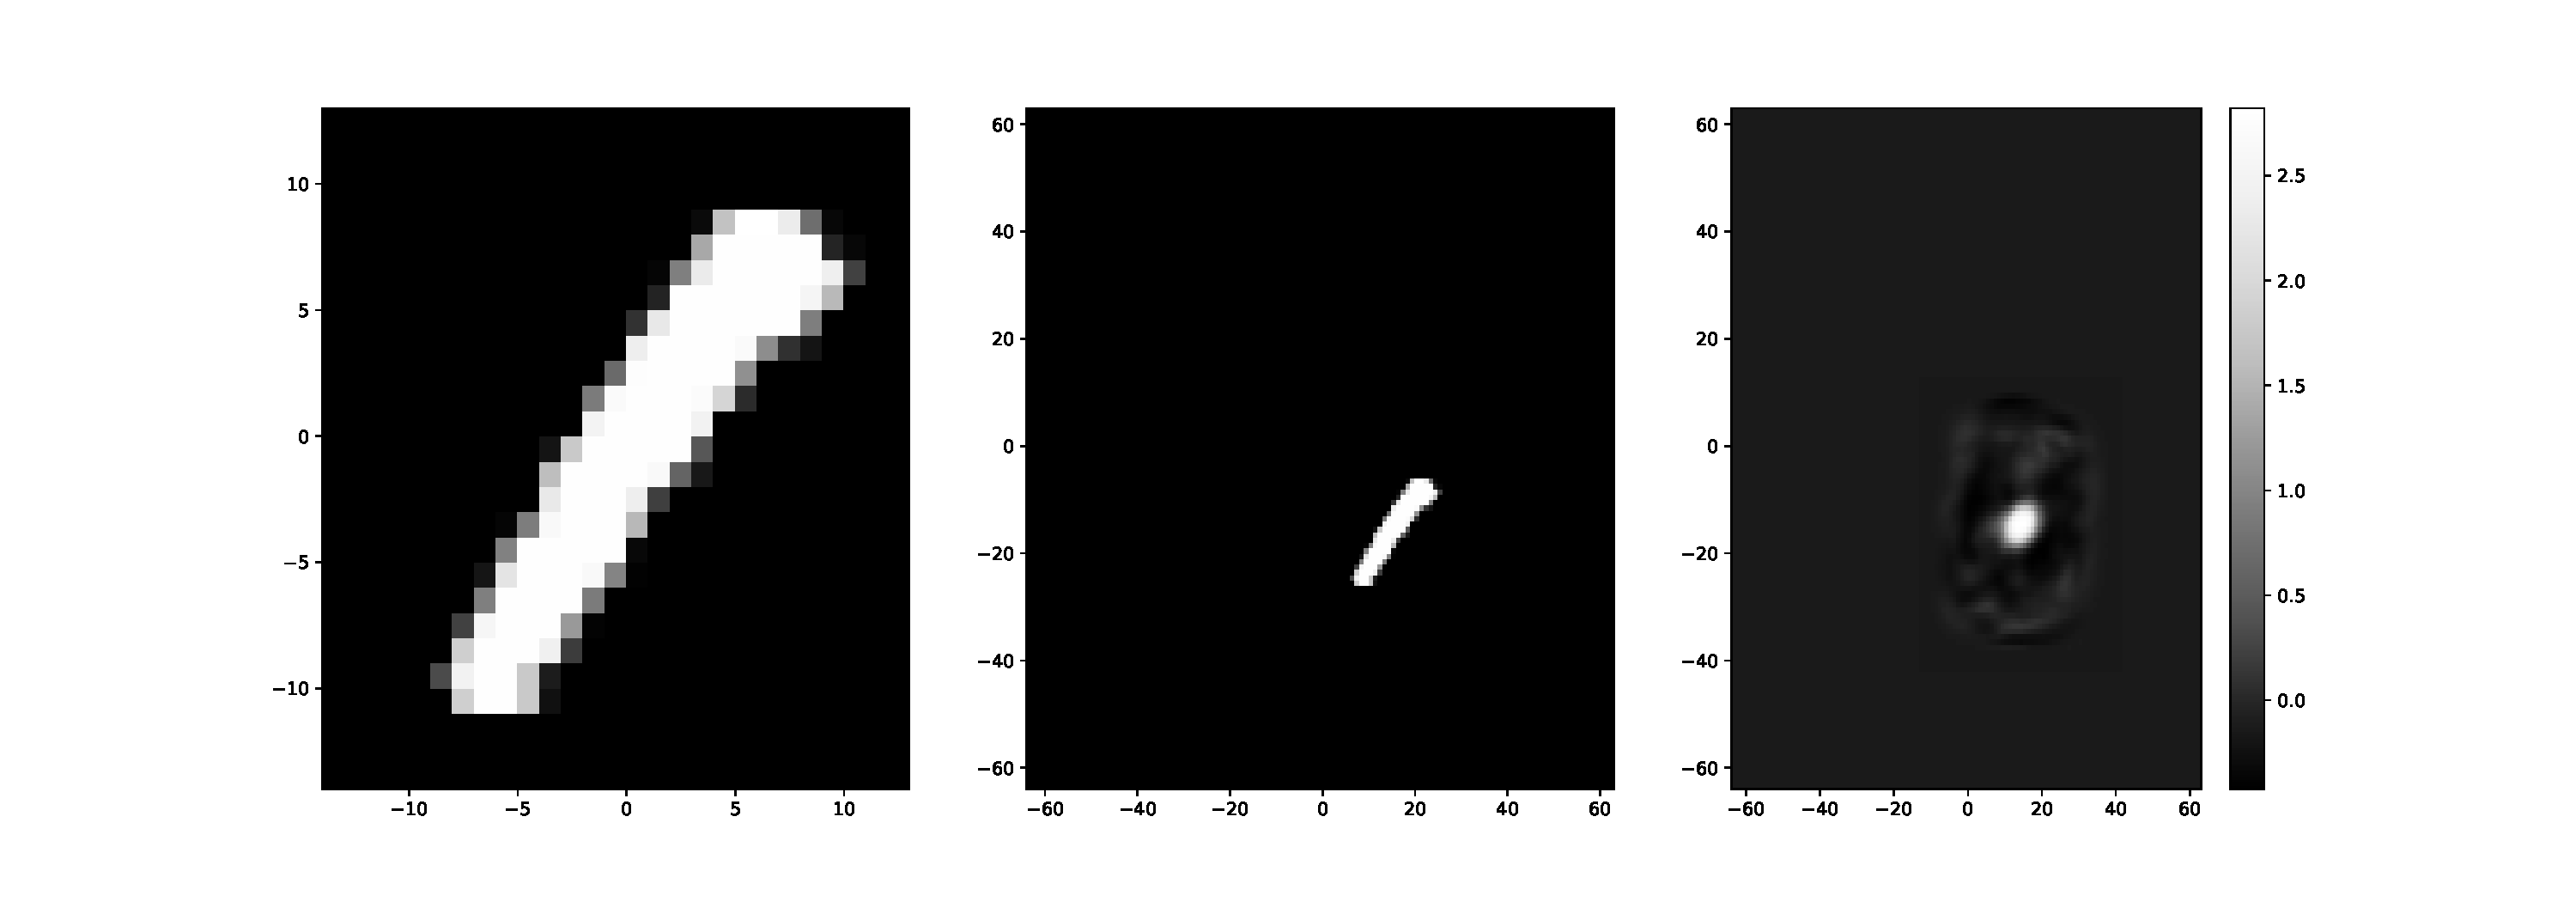
\includegraphics[scale=0.4]{Figures/couples_a-v}
\decoRule
\caption[Figure]{Illustration en cartes de chaleur de la construction automatique d'un couple stimulus/label par la modèle. L'emplacement du chiffre MNIST dans l'image $128\times 128$ pixels est choisi au hasard, et cette même position est reprise pour placer la carte de certitude dans l'autre image $128\times 128$ pixels}
\label{fig:couples}
\end{figure}

\begin{figure}[th]
\centering
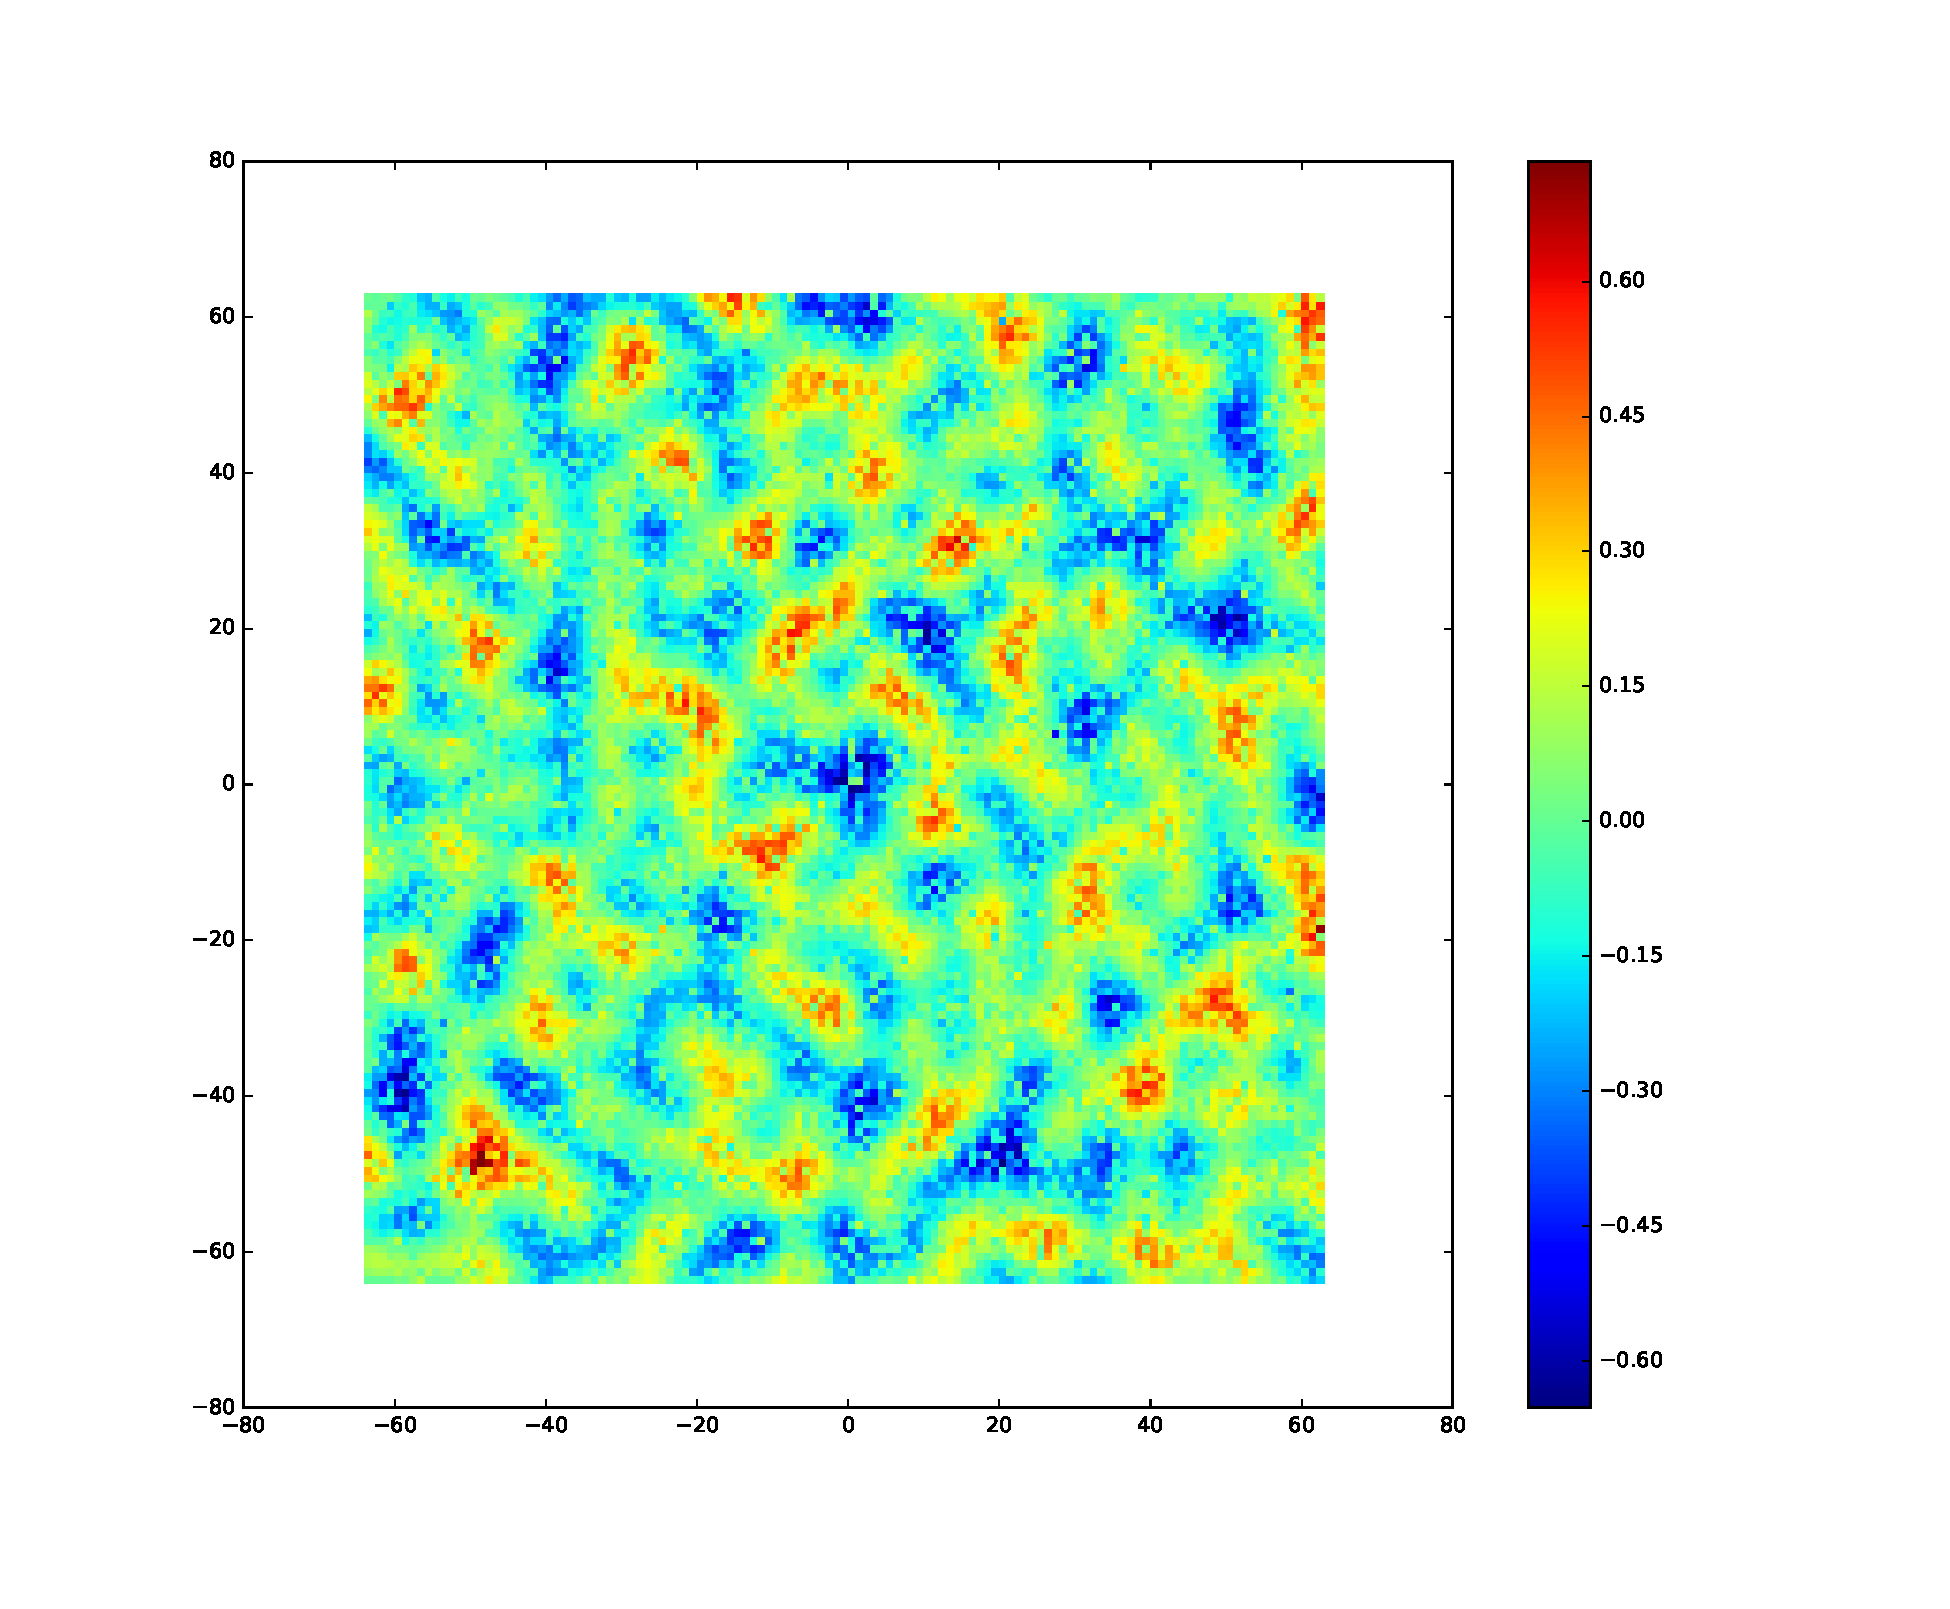
\includegraphics[scale=0.4]{Figures/perlin_noise}
\decoRule
\caption[Figure]{Reconstruction en carte de chaleur ($128\times 128$ pixels) d'un bruit Perlin généré automatiquement et aléatoirement \autocite{Perlin1985}}
\label{fig:perlin_noise}
\end{figure}

\begin{figure}[th]
\centering
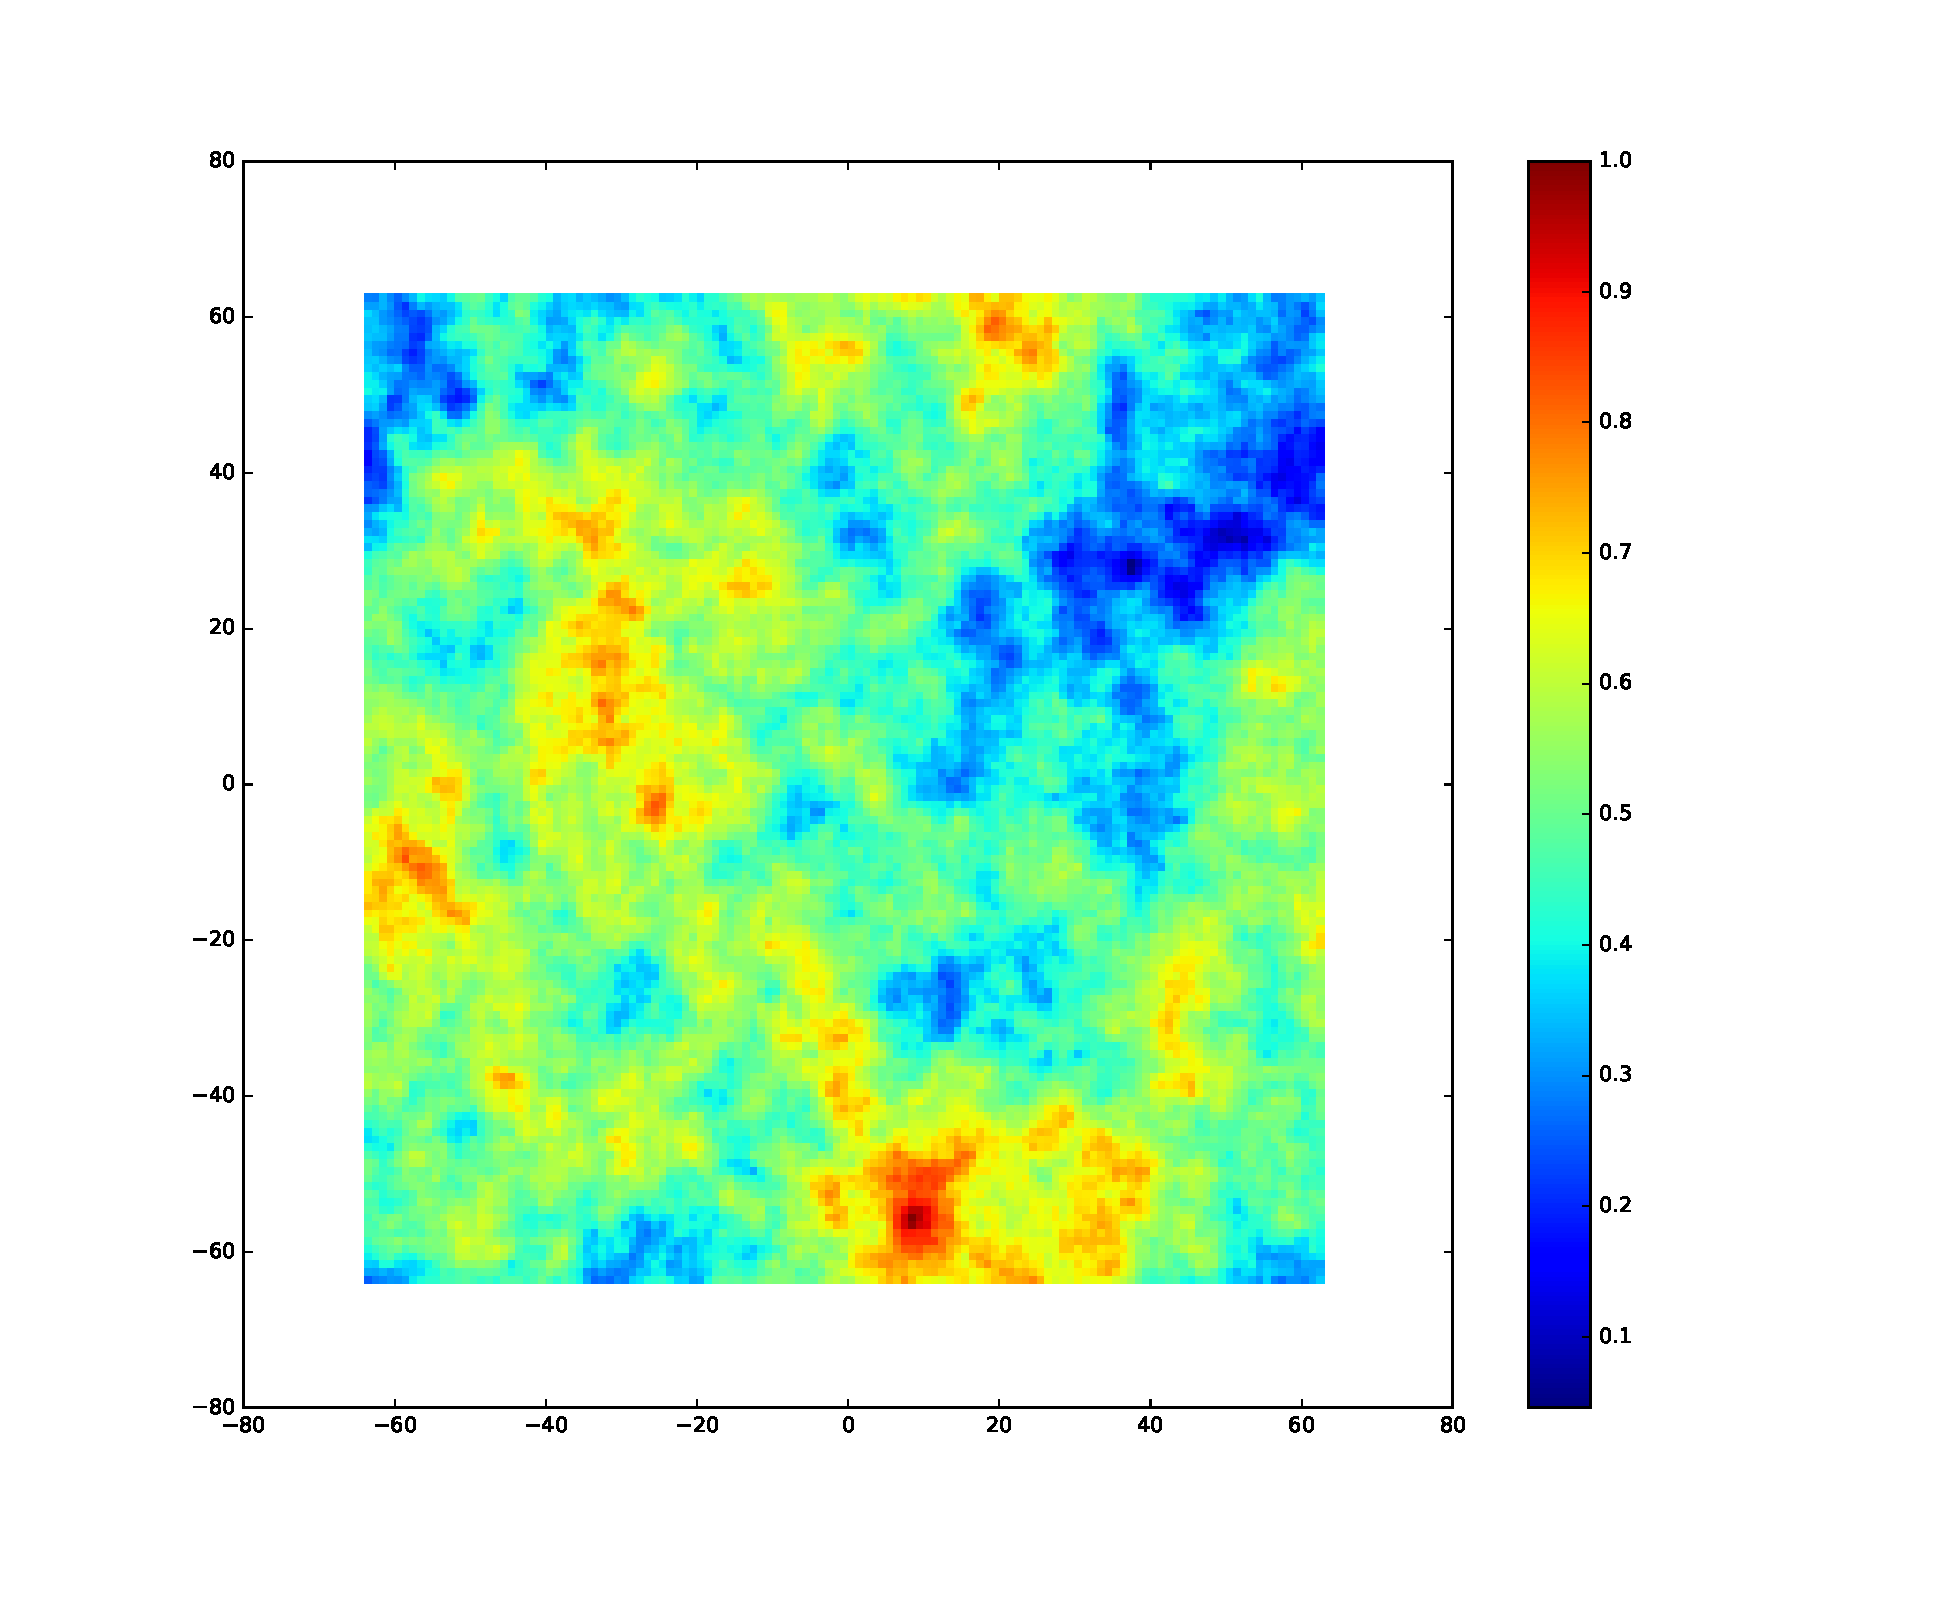
\includegraphics[scale=0.4]{Figures/motioncloud_noise}
\decoRule
\caption[Figure]{Reconstruction en carte de chaleur ($128\times 128$ pixels) d'un bruit MotionCloud généré automatiquement et aléatoirement \autocite{Leon2012}}
\label{fig:motioncloud_noise}
\end{figure}

\begin{figure}[th]
\centering
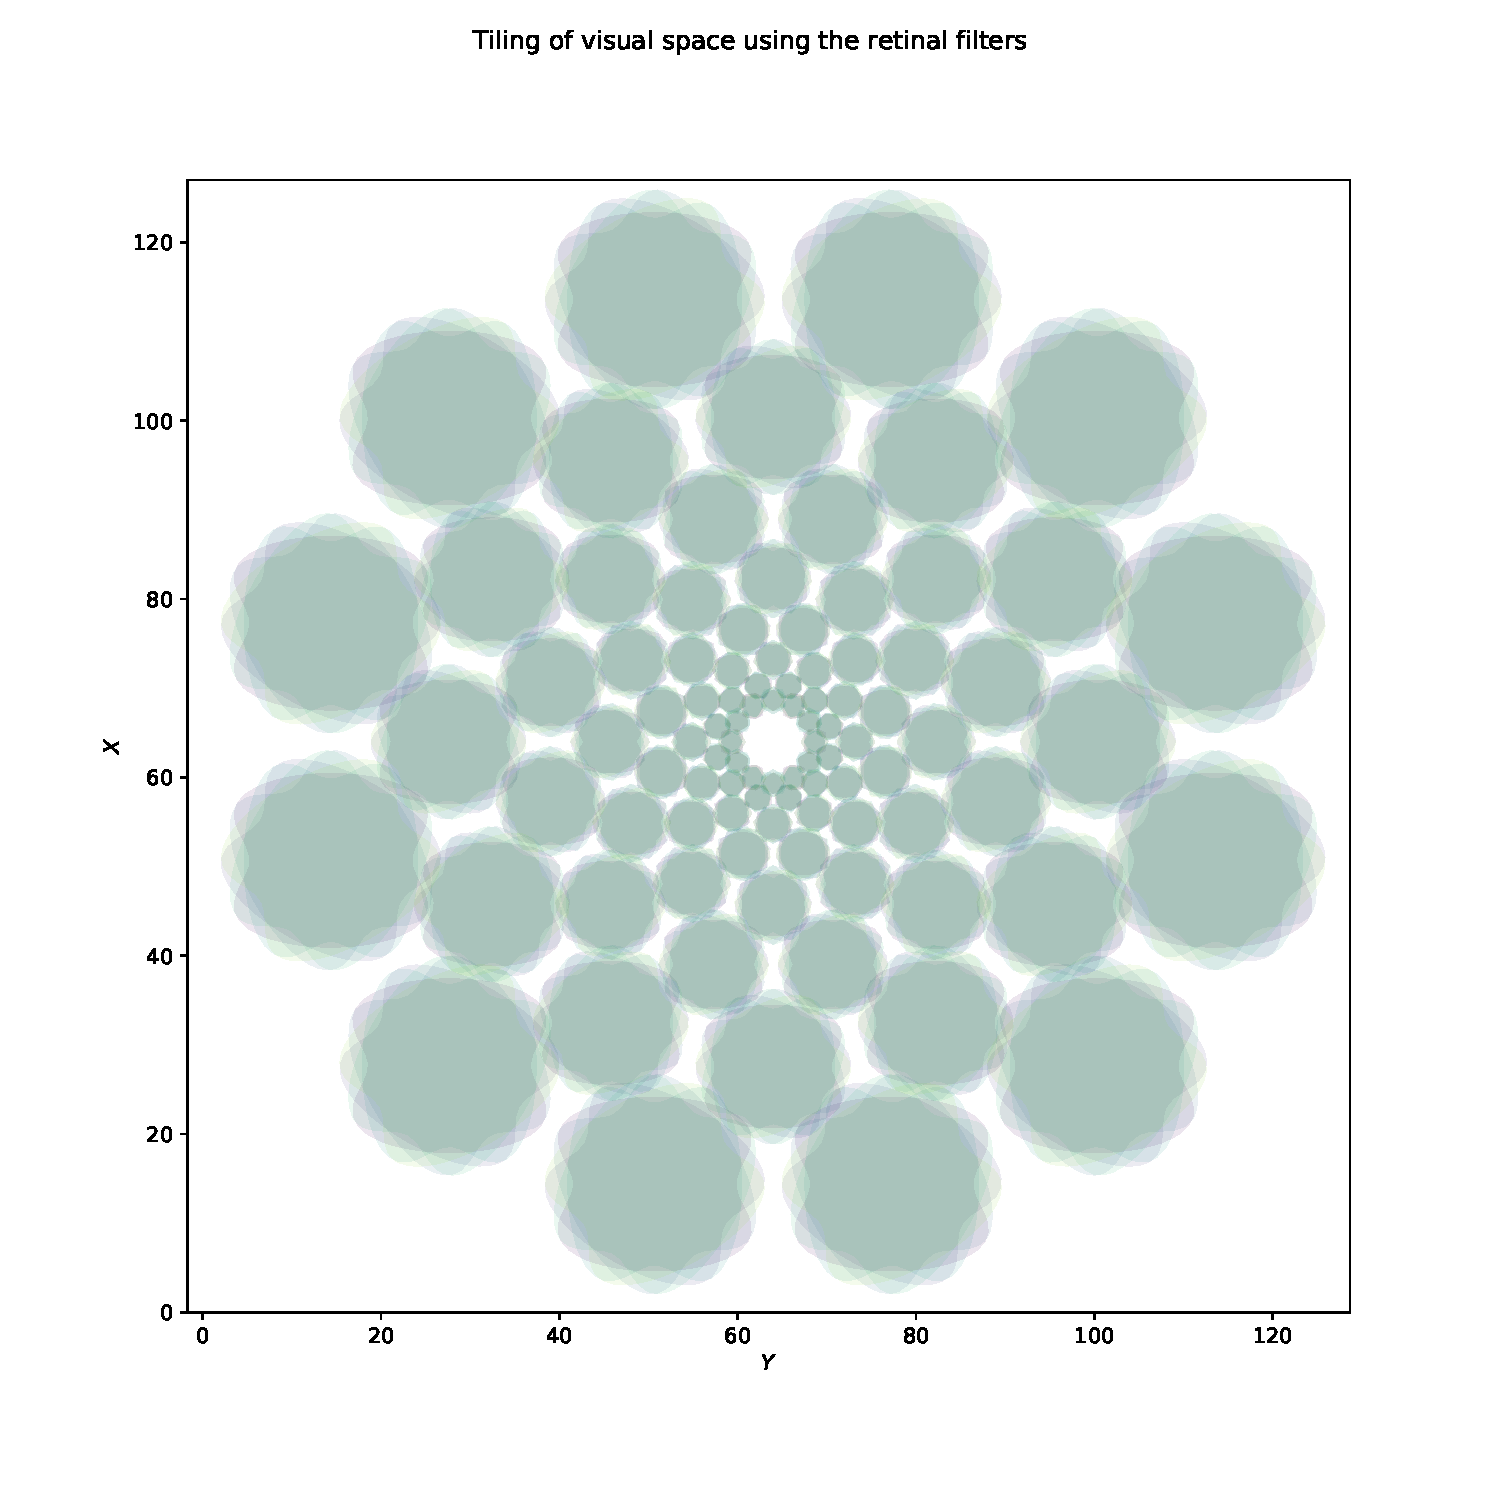
\includegraphics[scale=0.4]{Figures/retina_filter}
\decoRule
\caption[Figure]{Schéma ($128\times 128$ pixels) représentant le filtre LogPolaire pour les paramètres (theta=6, azimuth=12, eccentricity=8, phase=2, rho=1.61803). Chaque ovoïde représente un champs récepteur, modélisé par un filtre Gabor \autocite{Freeman2011}}
\label{fig:logpol_filter}
\end{figure}

\begin{figure}[th]
\centering
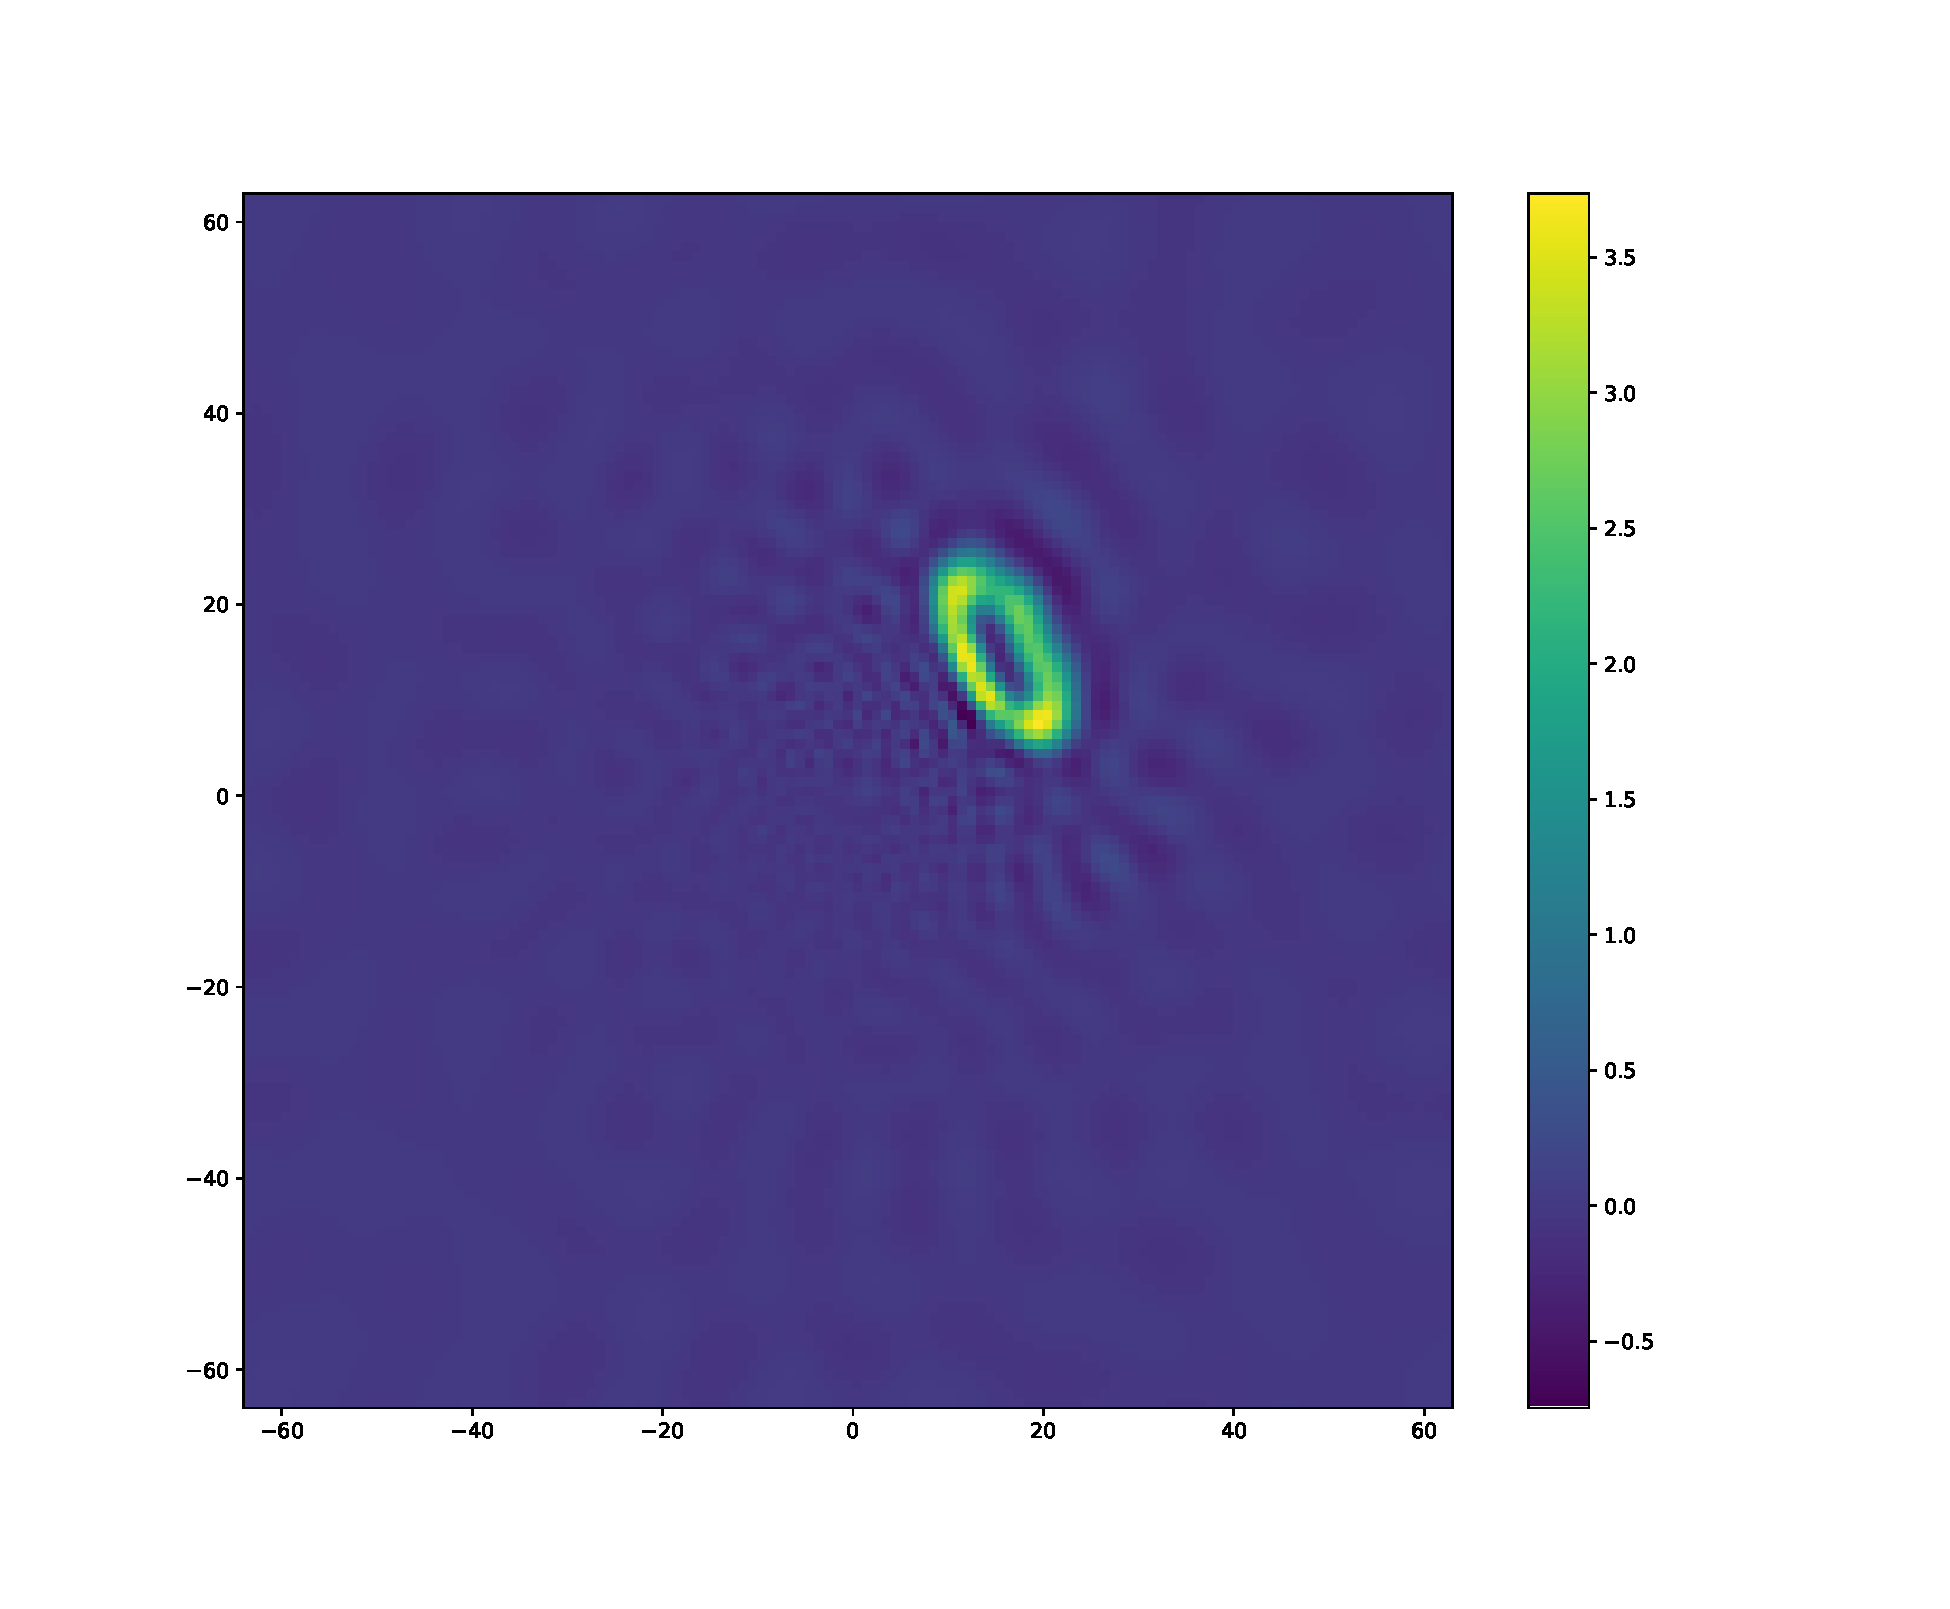
\includegraphics[scale=0.4]{Figures/mnist_128_LP_nonoise}
\decoRule
\caption[Figure]{Reconstruction en carte de chaleur ($128\times 128$ pixels) d'un stimulus non-bruité après passage dans le filtre rétinien LogPolaire}
\label{fig:mnist_128_LP_nonoise}
\end{figure}

\begin{figure}[th]
\centering
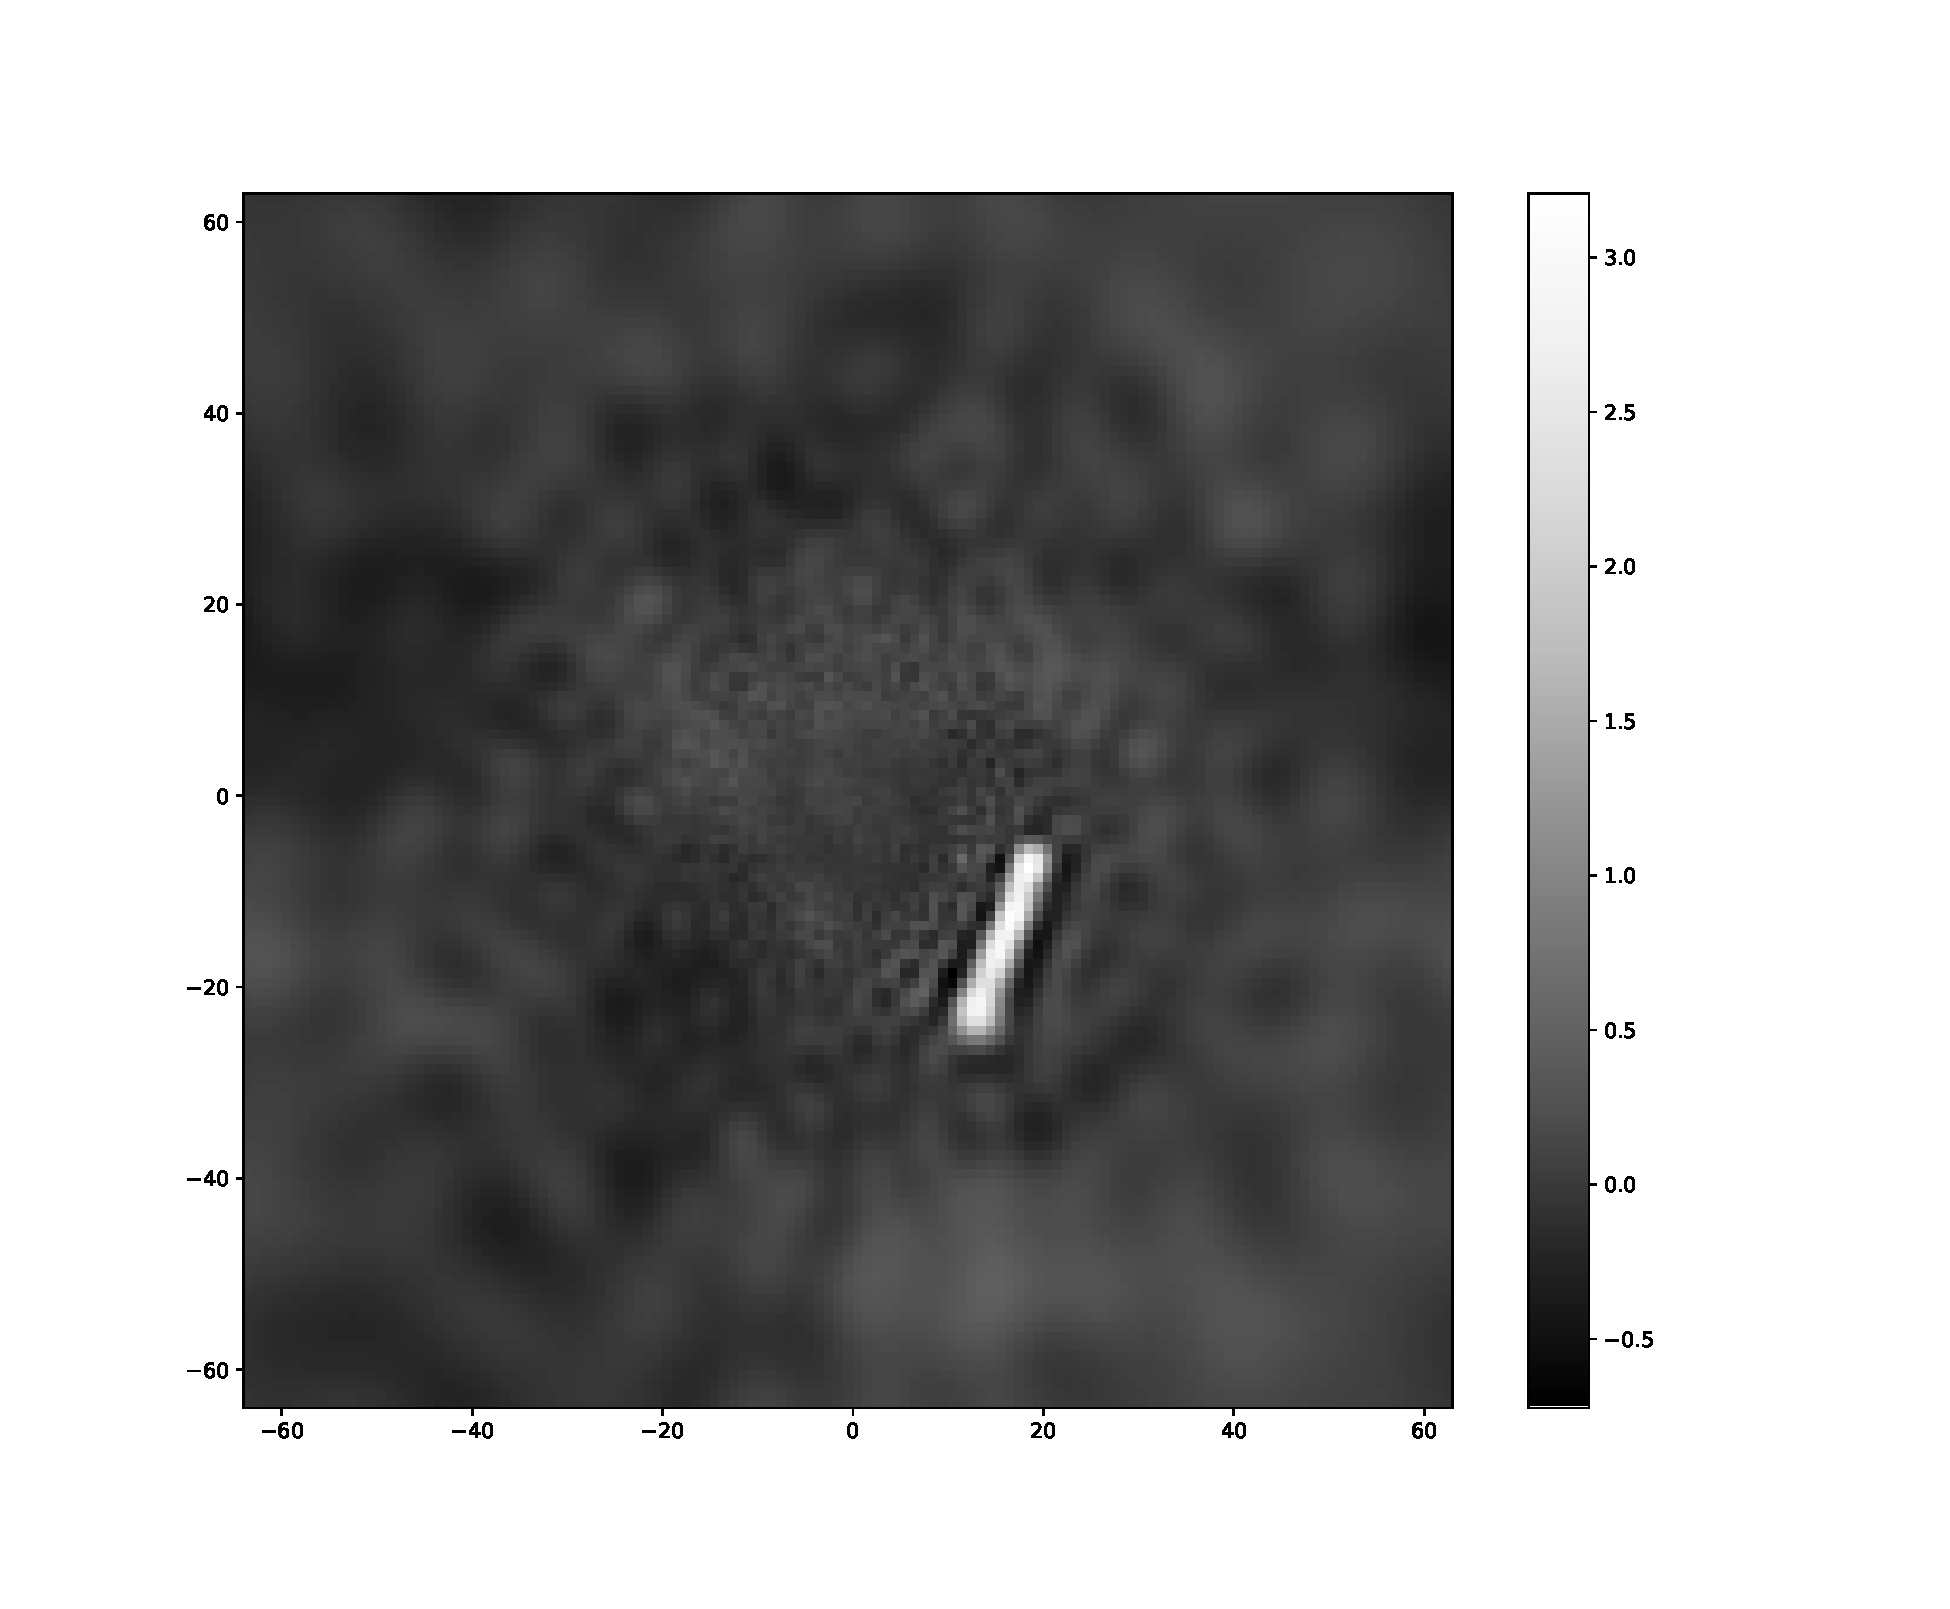
\includegraphics[scale=0.4]{Figures/mnist_128_LP_noise}
\decoRule
\caption[Figure]{Reconstruction en carte de chaleur ($128\times 128$ pixels) d'un stimulus bruité par la méthode MotionCloud après passage dans le filtre rétinien LogPolaire}
\label{fig:mnist_128_LP_MotionCloud}
\end{figure}

\begin{figure}[th]
\centering
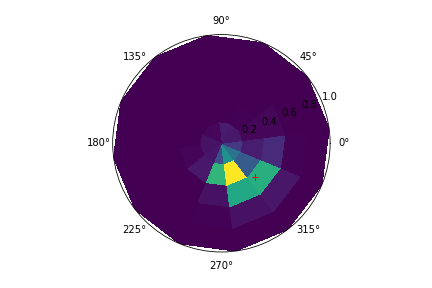
\includegraphics[scale=0.4]{Figures/mnist_log_nonoise}
\decoRule
\caption[Figure]{Reconstruction en graphique logarithmique d'un stimulus non-bruité après passage dans le filtre rétinien LogPolaire. La croix rouge représente la position du stimulus}
\label{fig:mnist_log_nonoise}
\end{figure}

\begin{figure}[th]
\centering
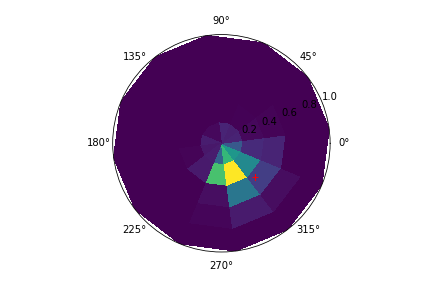
\includegraphics[scale=0.4]{Figures/mnist_log_motioncloud}
\decoRule
\caption[Figure]{Reconstruction en graphique logarithmique d'un stimulus bruité par la méthode MotionCloud après passage dans le filtre rétinien LogPolaire. La croix rouge représente la position du stimulus}
\label{fig:mnist_log_motioncloud}
\end{figure}

\begin{figure}[th]
\centering
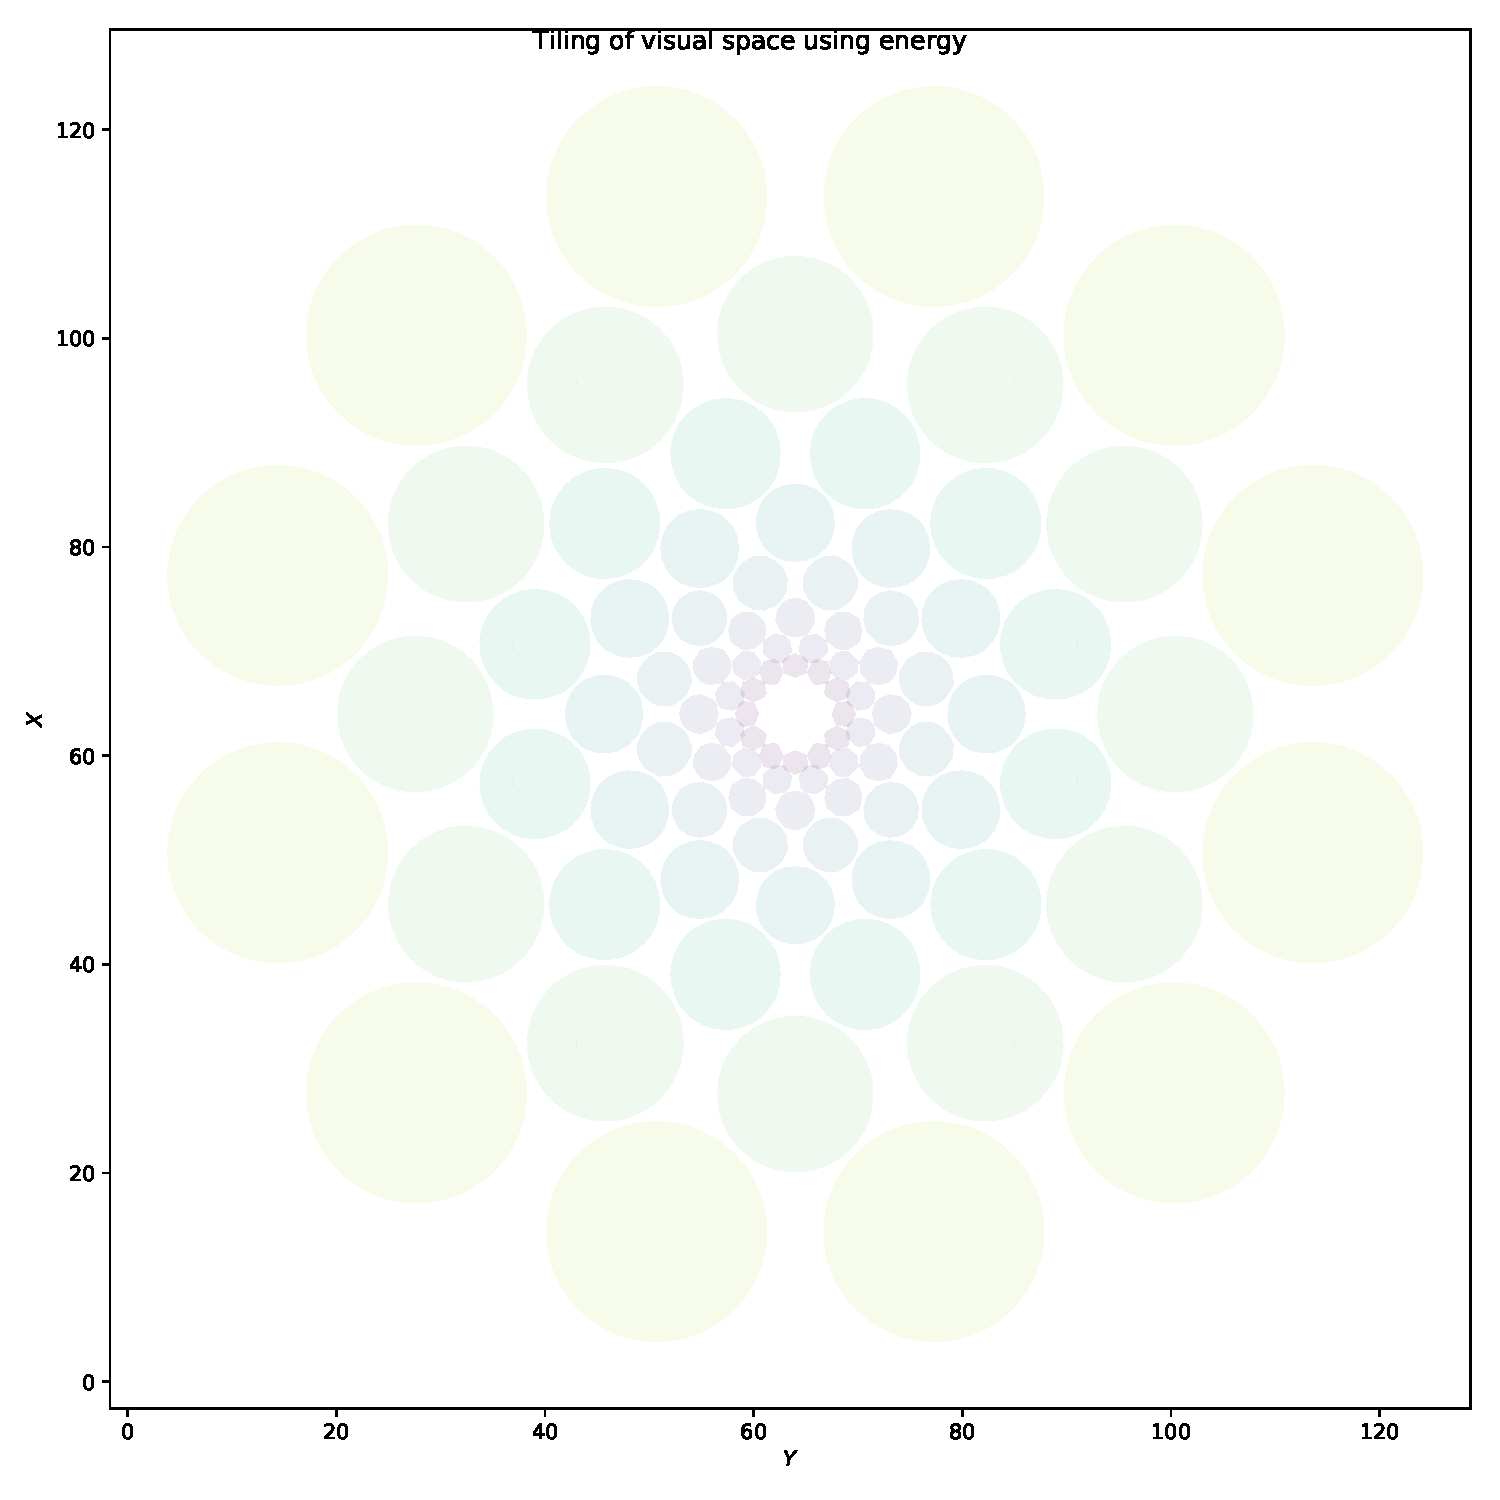
\includegraphics[scale=0.4]{Figures/colliculus_filter}
\decoRule
\caption[Figure]{Schéma ($128\times 128$ pixels) représentant le filtre LogPolaire énergétique pour les paramètres (azimuth=12, eccentricity=8, rho=1.61803). Chaque cercle représente un champ récepteur}
\label{fig:energy_filter}
\end{figure}

\begin{figure}[th]
\centering
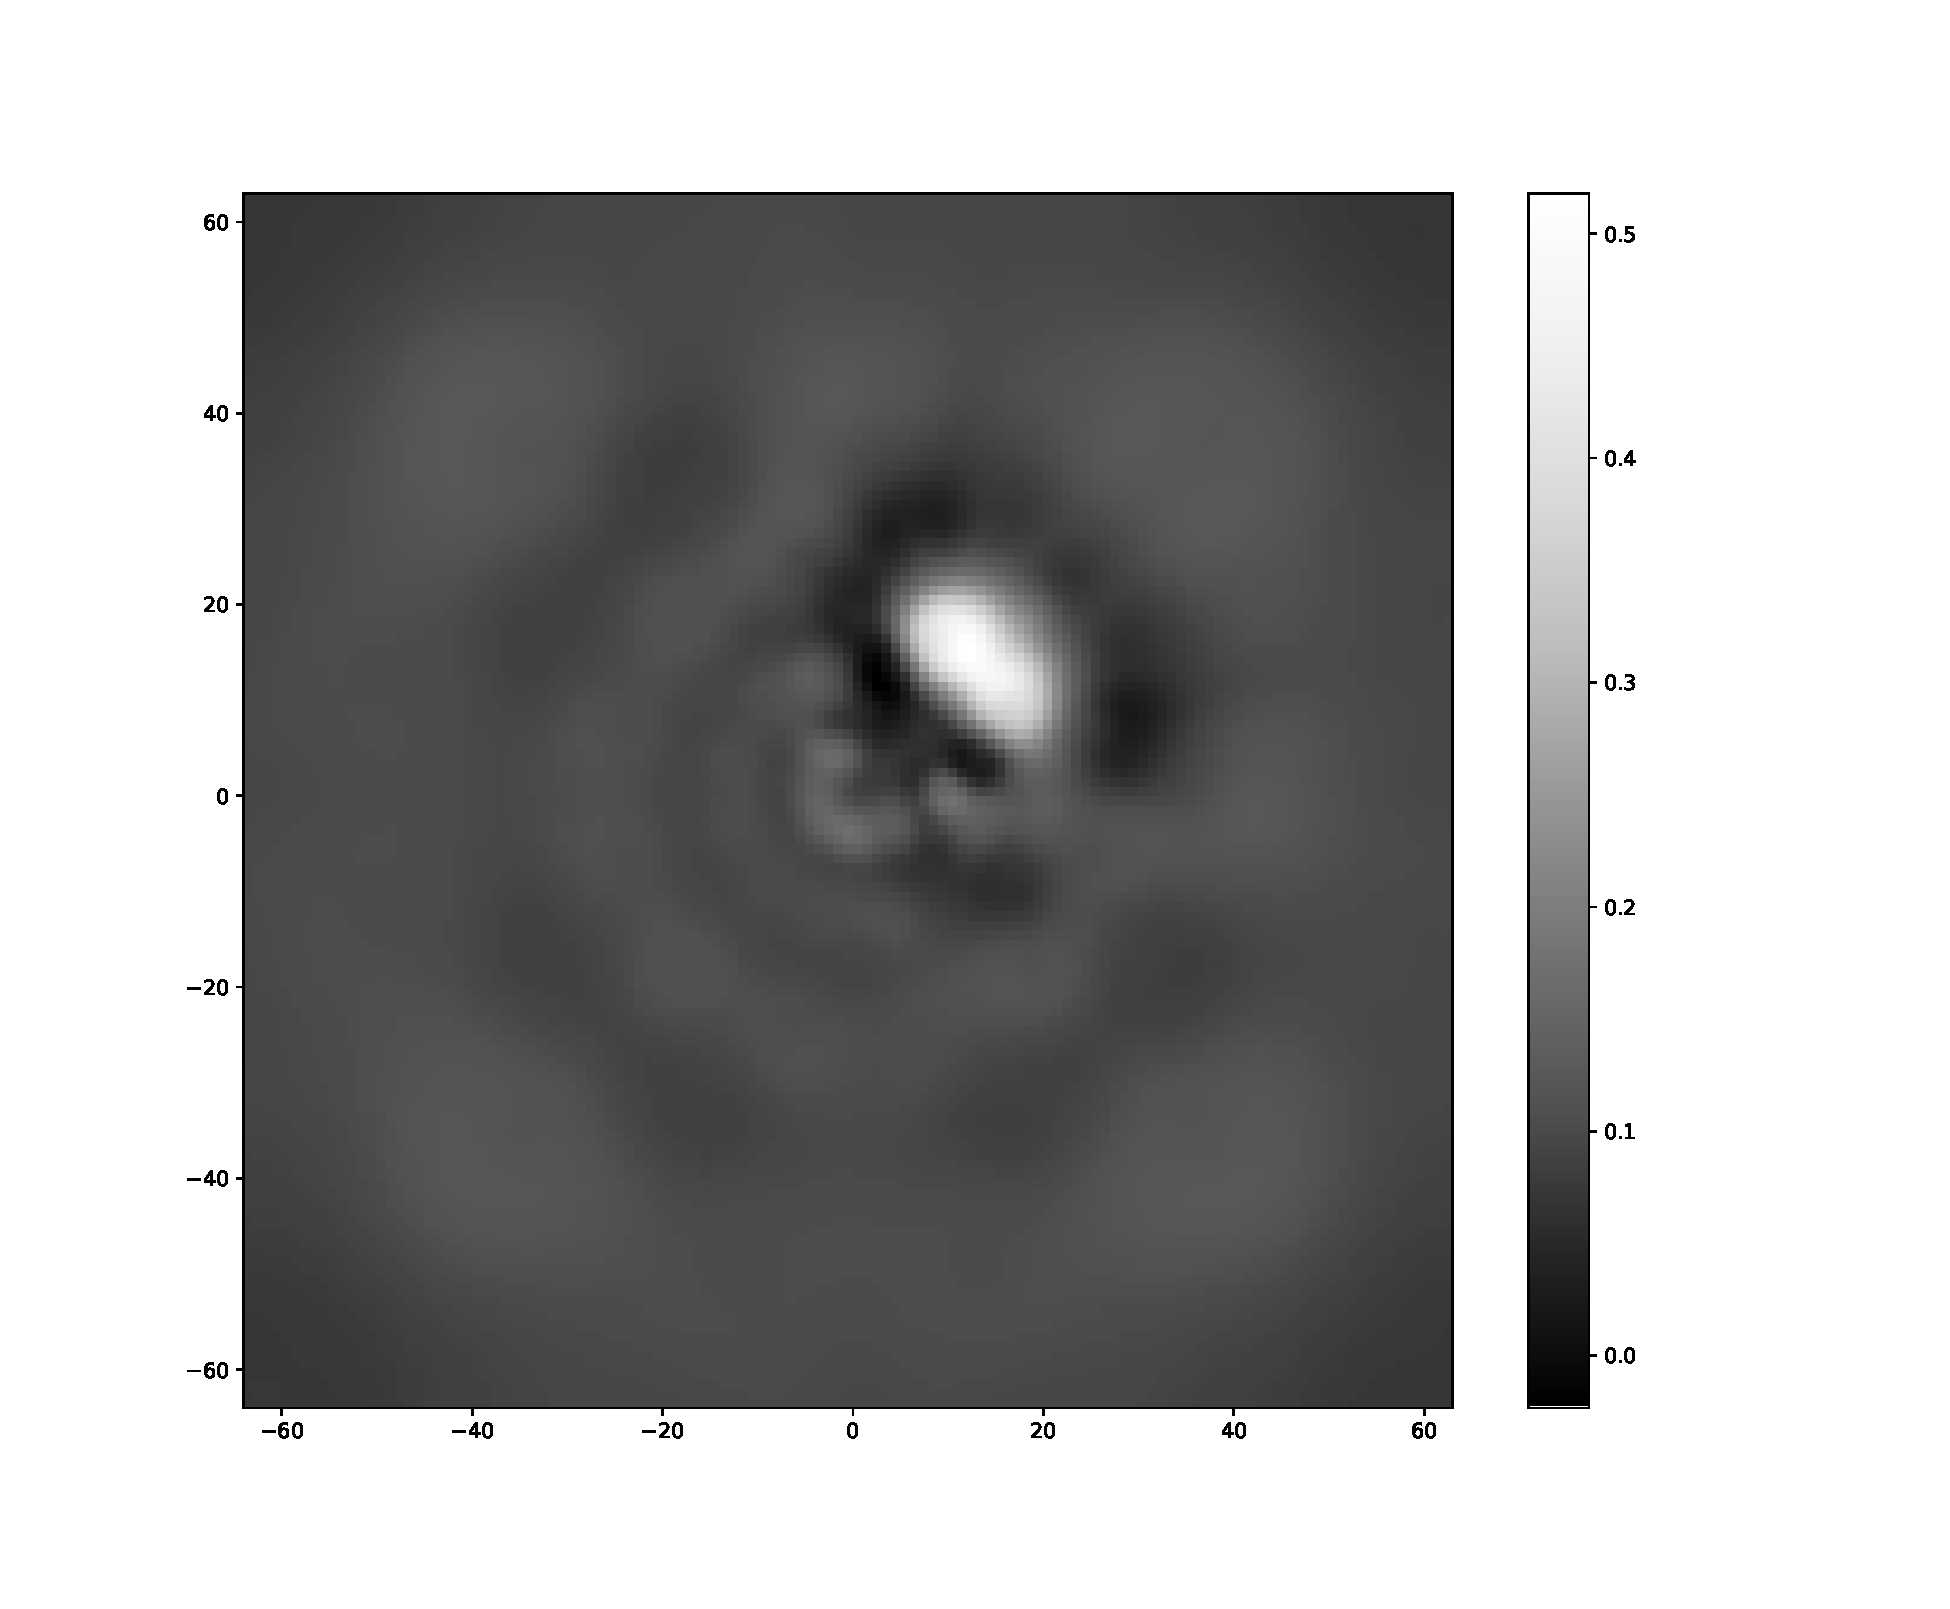
\includegraphics[scale=0.4]{Figures/accuracy_colliculus}
\decoRule
\caption[Figure]{Reconstruction en carte de chaleur ($128\times 128$ pixels) de la carte de certitude après passage dans le filtre rétinien LogPolaire}
\label{fig:accuracy_128_LP}
\end{figure}

\begin{figure}[th]
\centering
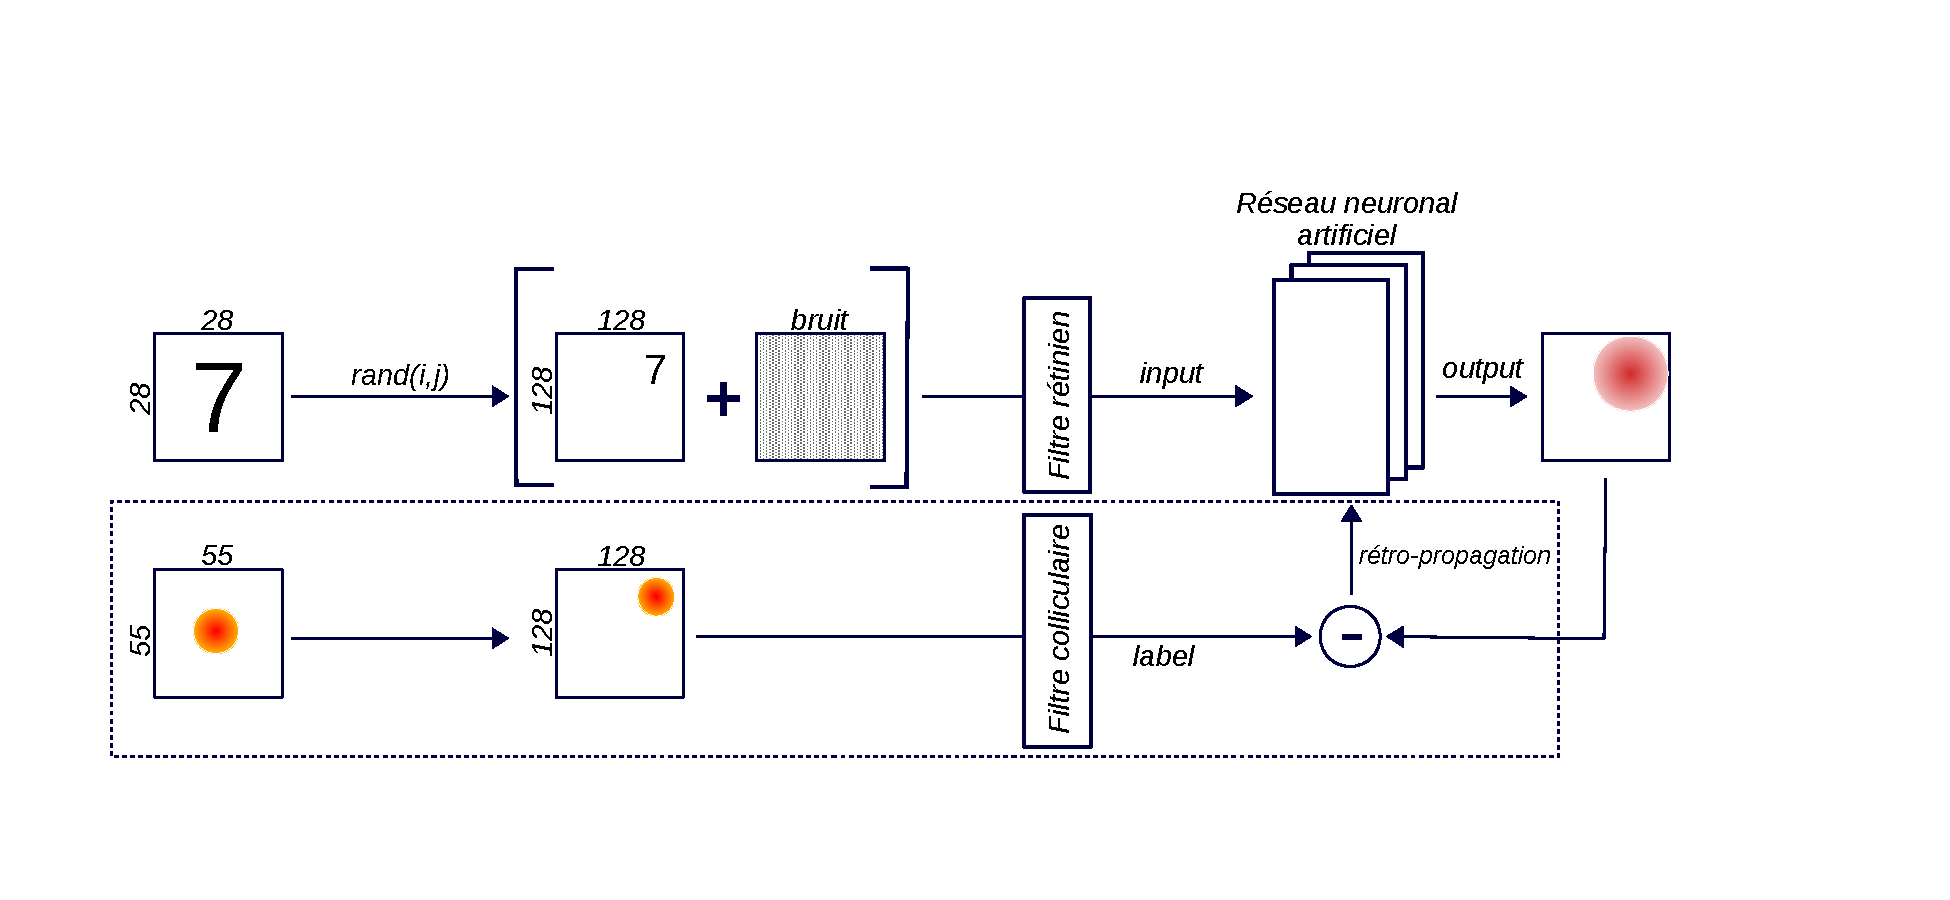
\includegraphics[scale=0.65]{Figures/Model}
\decoRule
\caption[Figure]{Schéma décrivant les étapes nécessaires à la production de nos entrées (ou \textit{input}) et de nos labels, puis celles pour que notre modèle réalise des prédictions (sorties ou \textit{output}) de la position des stimuli. La partie entourée en pointillés, correspondant à la production et l'intégration du label, n'est réalisée que lors de la phase d'apprentissage}
\label{fig:model}
\end{figure}

%%%%% Résultats %%%%%

\begin{figure}[th]
\centering
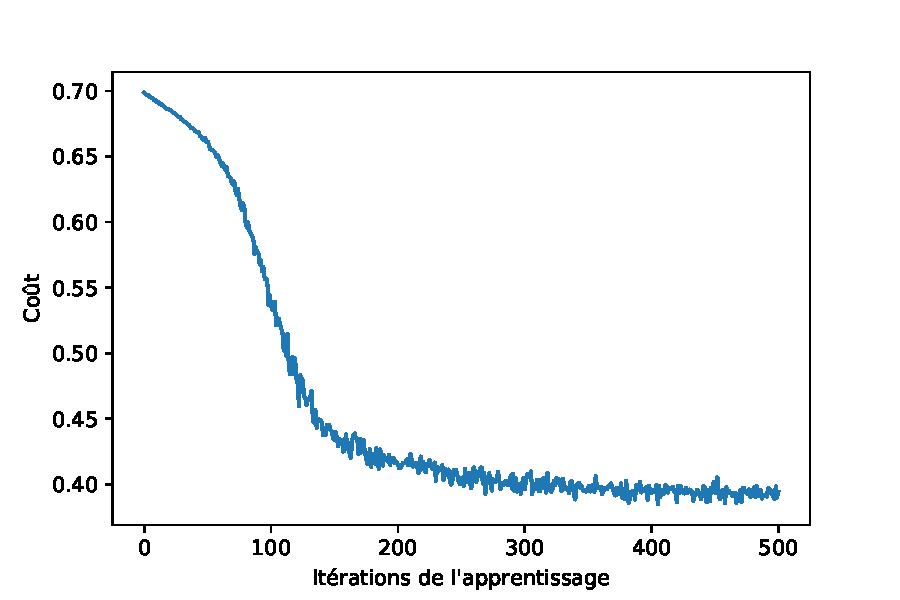
\includegraphics[scale=0.8]{Figures/losses}
\decoRule
\caption[Figure]{Variations de la valeur de coût du modèle au cours de la première époque d'apprentissage, pour un paramètre d'apprentissage alpha$=0.05$}
\label{fig:losses}
\end{figure}

\begin{figure}[th]
\centering
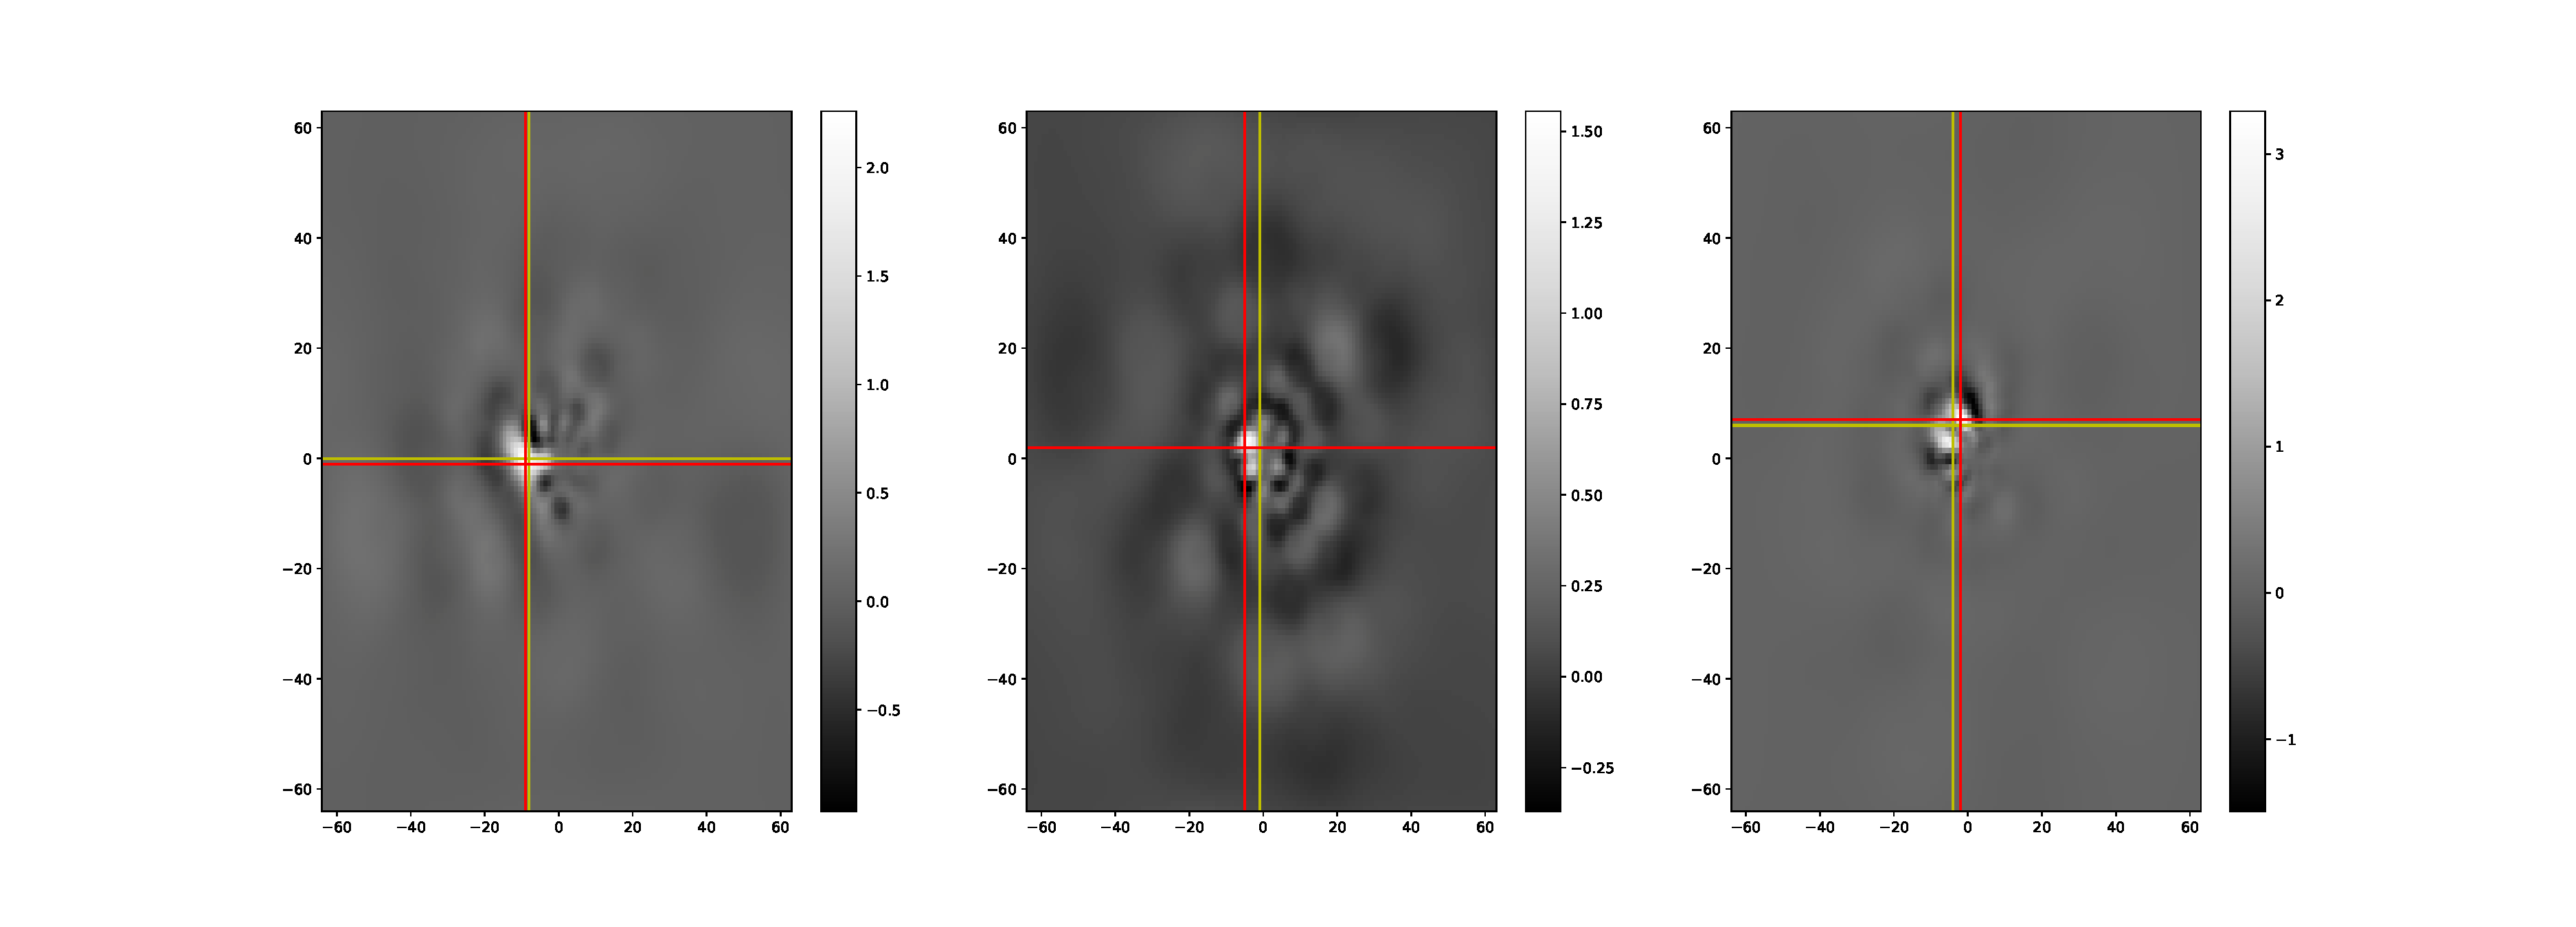
\includegraphics[scale=0.325]{Figures/prediction}
\decoRule
\caption[Figure]{Reconstructions en carte de chaleur ($128\times 128$ pixels) de la sortie du modèle lors de la phase d'évaluation. Chaque figure représente un essai différent. Les croix jaunes représentent la position réelle de la cible dans l'environnement visuel, tandis que les croix rouges représentent sa position prédite par le modèle}
\label{fig:prediction}
\end{figure}
